\newcommand{\FigSensMuMomentum}{%
\begin{figure}[bt]
\centering 
%\fbox{
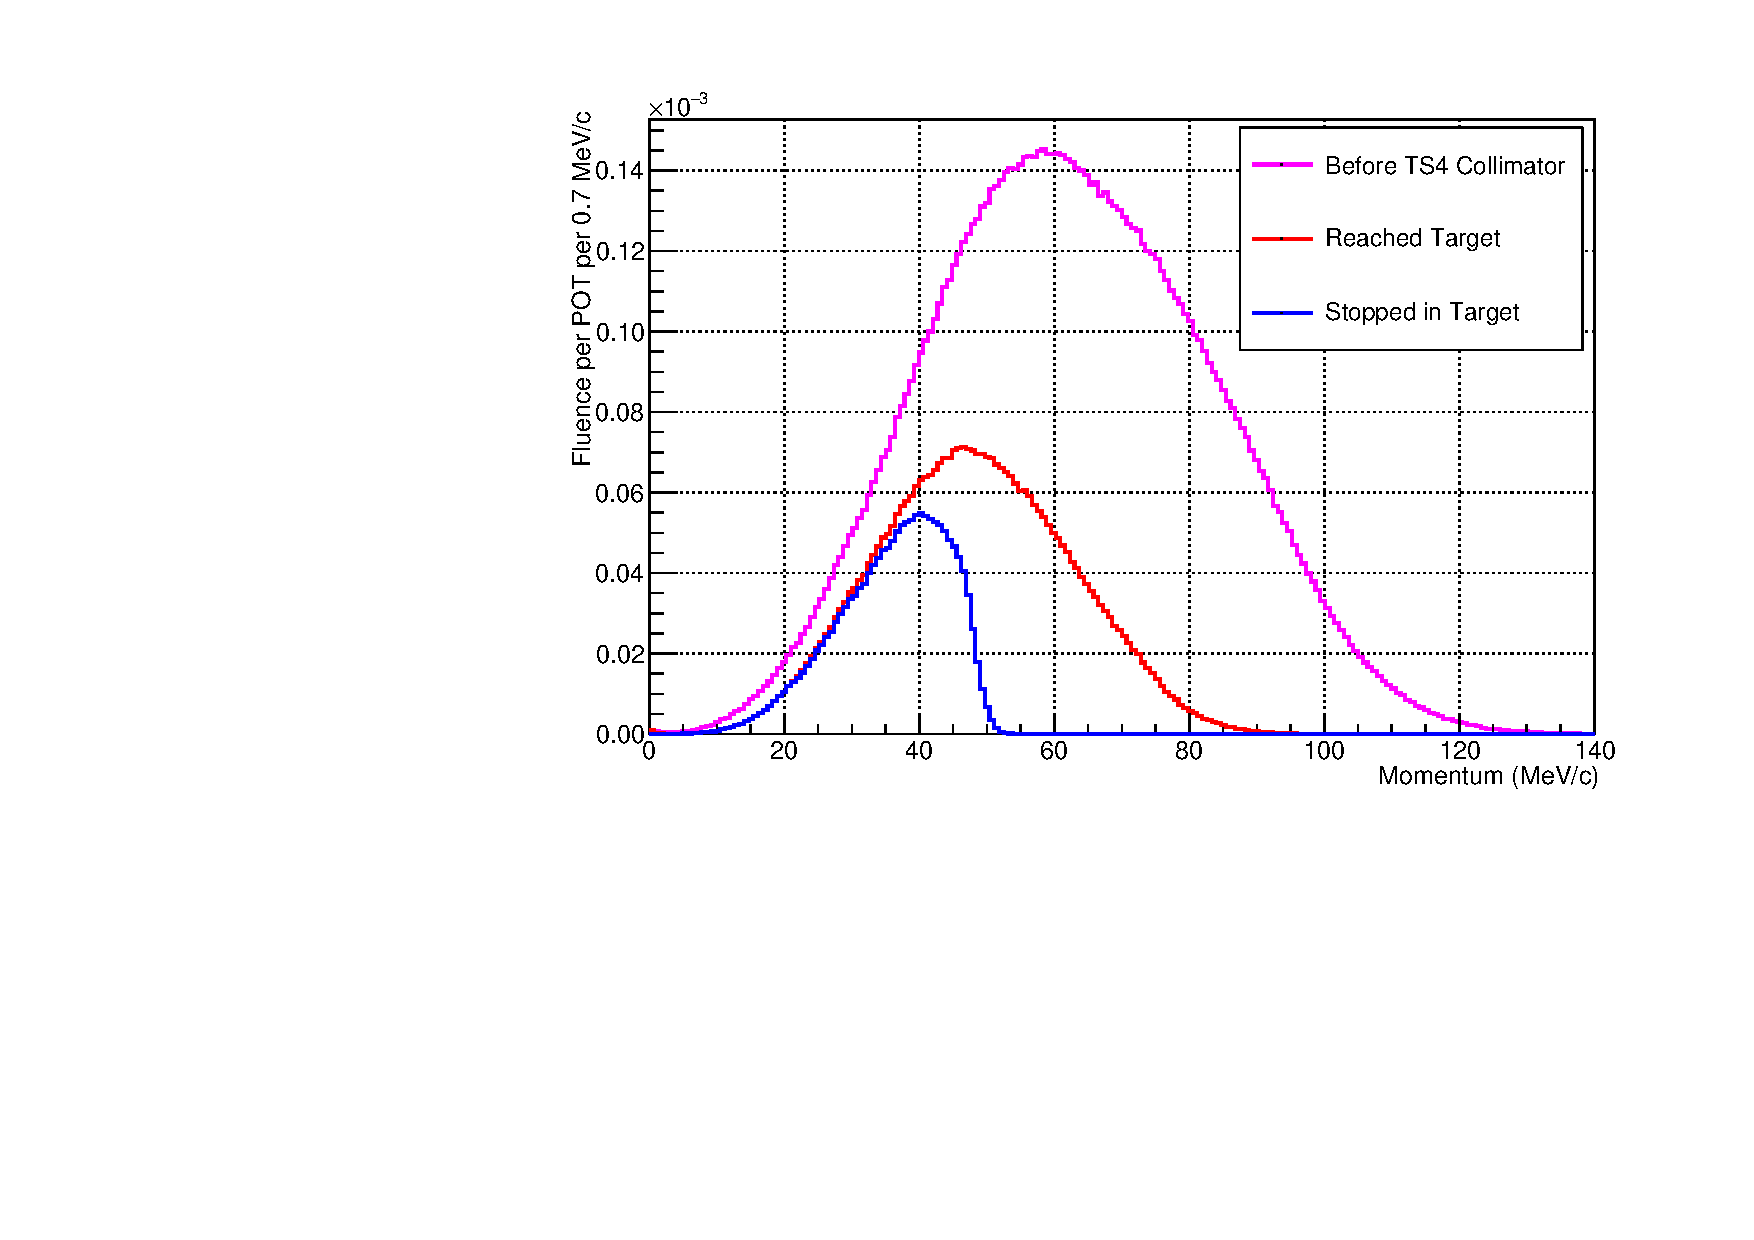
\includegraphics[width=0.8\textwidth,trim=0.5cm 0.1cm 1.5cm 0.8cm,clip]{figs/sensitivity/Muon_momentum.pdf}
%}
\caption{\figlabel{sense:muMomenta}
The Momentum and rates of muons reaching the final beam collimator, the stopping target, and actually stopping in the target.
It can be seen how the present target geometry is unable to stop muons of greater than around 50~MeV/c.
}
\end{figure}\xspace}

\newcommand{\FigSensMuStopsTwoD}{%
\begin{figure}[tb]
\centering 
\subfloat[\figlabel{sense:stops:XZ}X-Z plane]{
        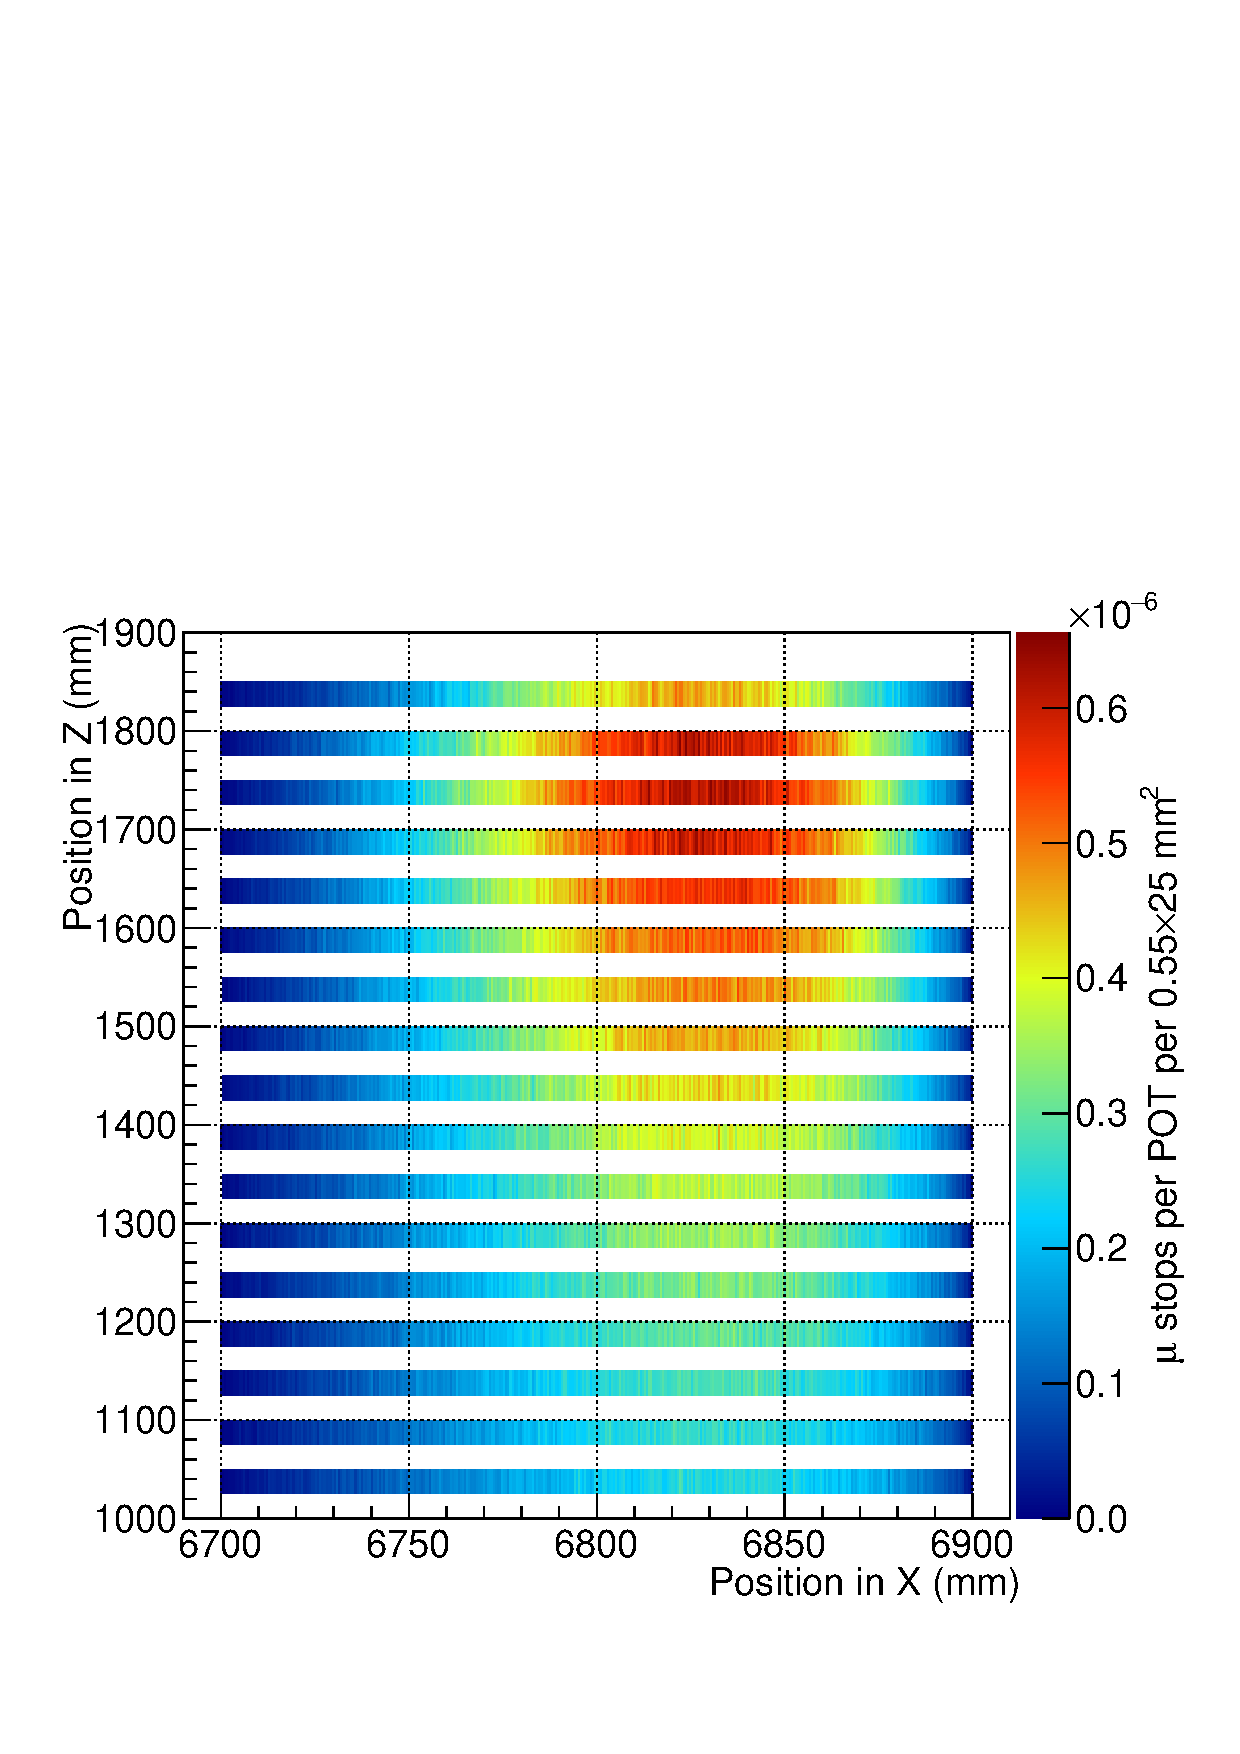
\includegraphics[width=0.33\textwidth,trim=0.3cm 1.5cm 0.7cm 1.2cm,clip]{figs/sensitivity/MuStops_2D_XZ.pdf}}
\subfloat[\figlabel{sense:stops:XY}X-Y plane]{
	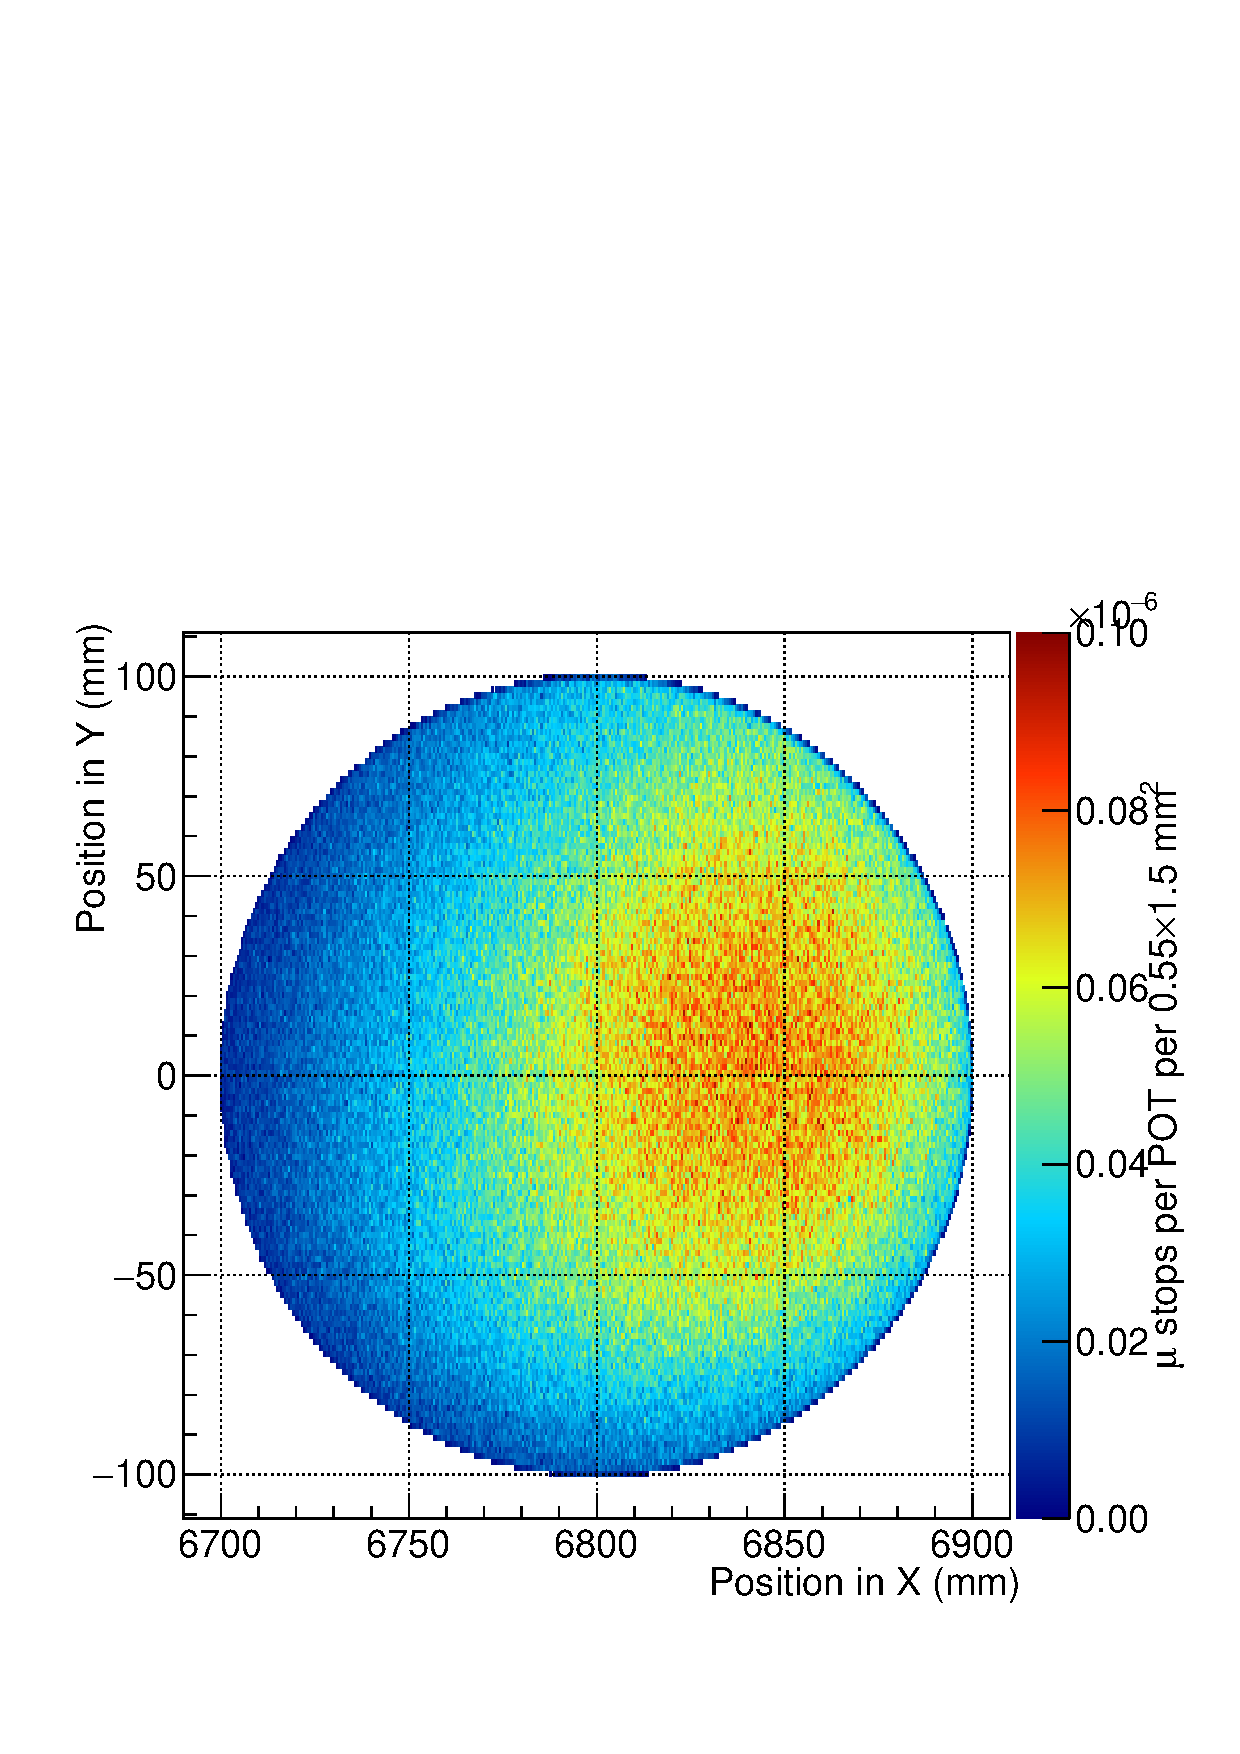
\includegraphics[width=0.33\textwidth,trim=0.3cm 1.5cm 0.7cm 1.2cm,clip]{figs/sensitivity/MuStops_2D_XY.pdf}}
\subfloat[\figlabel{sense:stops:ZY}Z-Y plane]{
	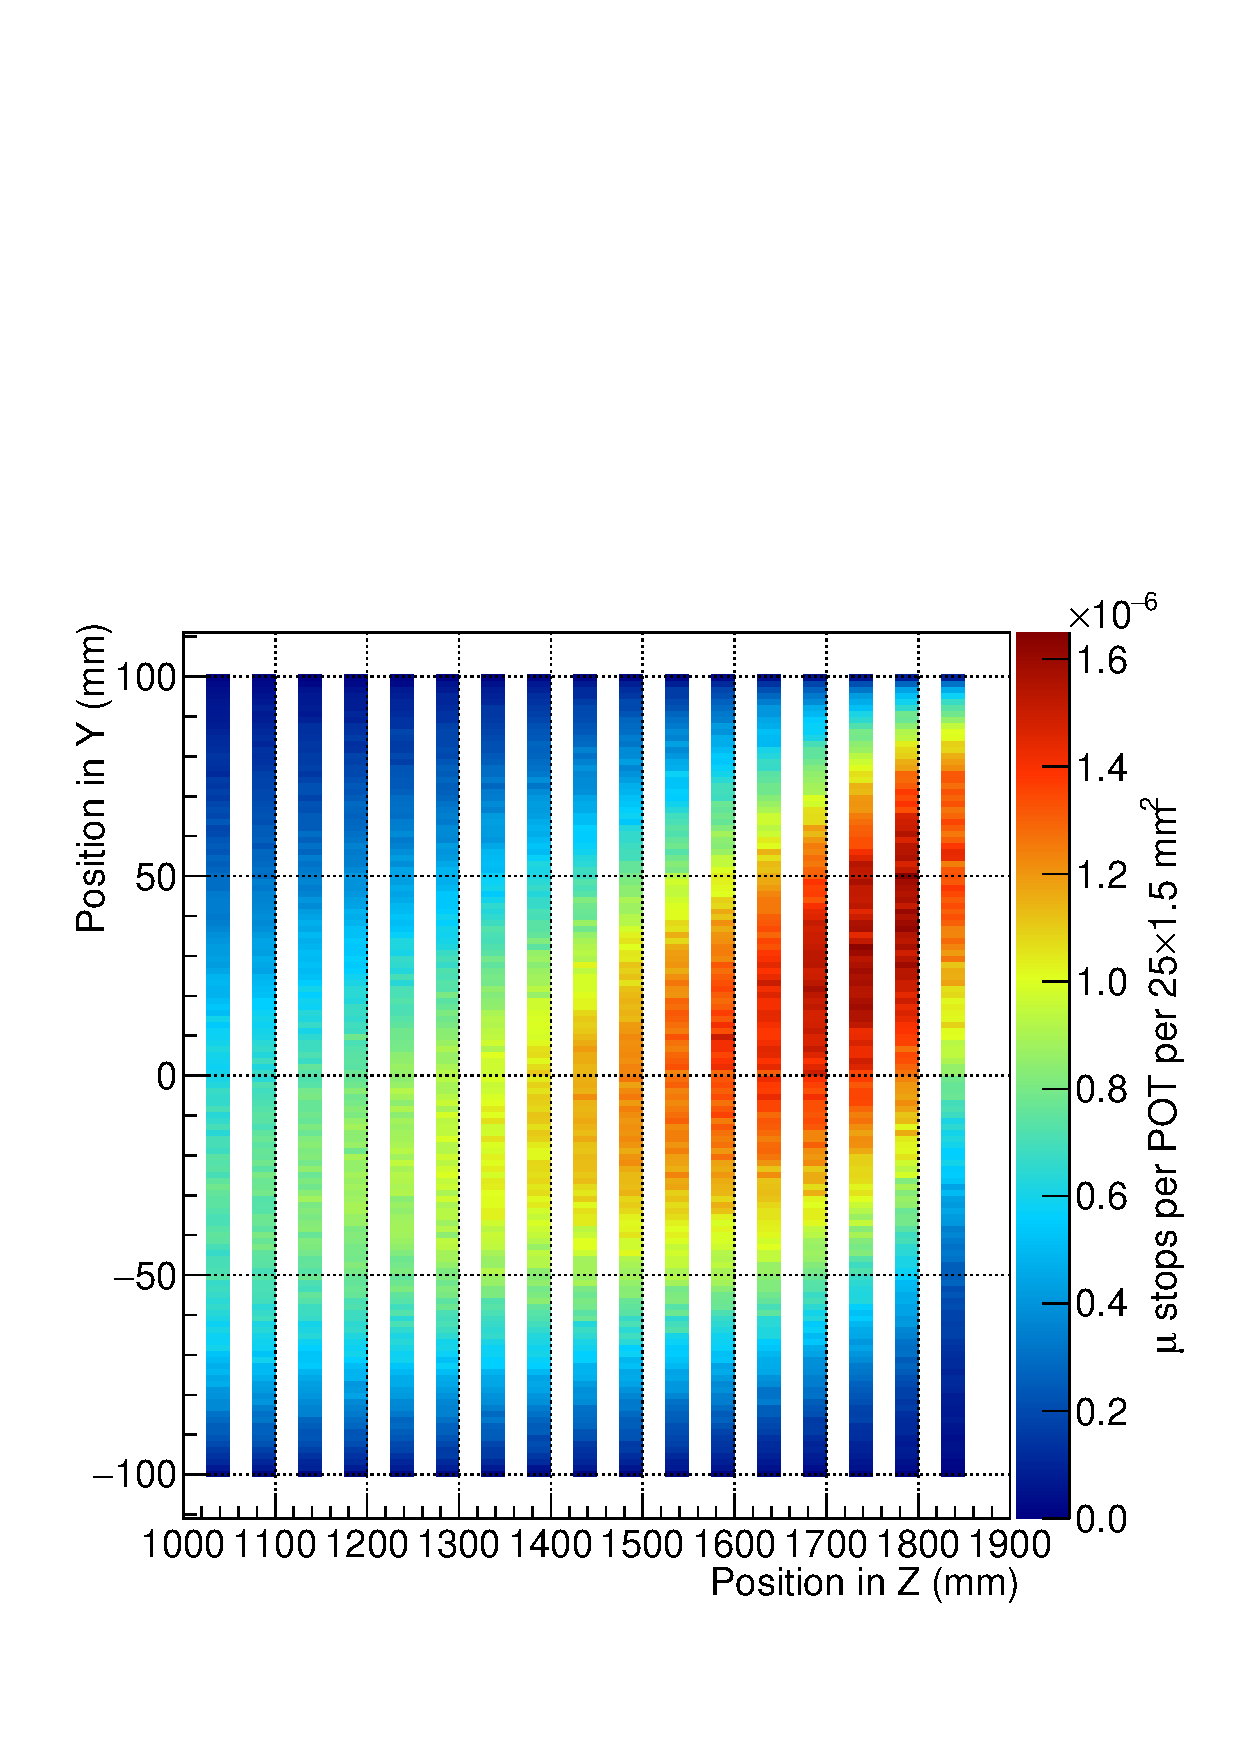
\includegraphics[width=0.33\textwidth,trim=0.3cm 1.5cm 0.7cm 1.2cm,clip]{figs/sensitivity/MuStops_2D_ZY.pdf}}
\\
\subfloat[\figlabel{sense:stops:X}X axis]{
	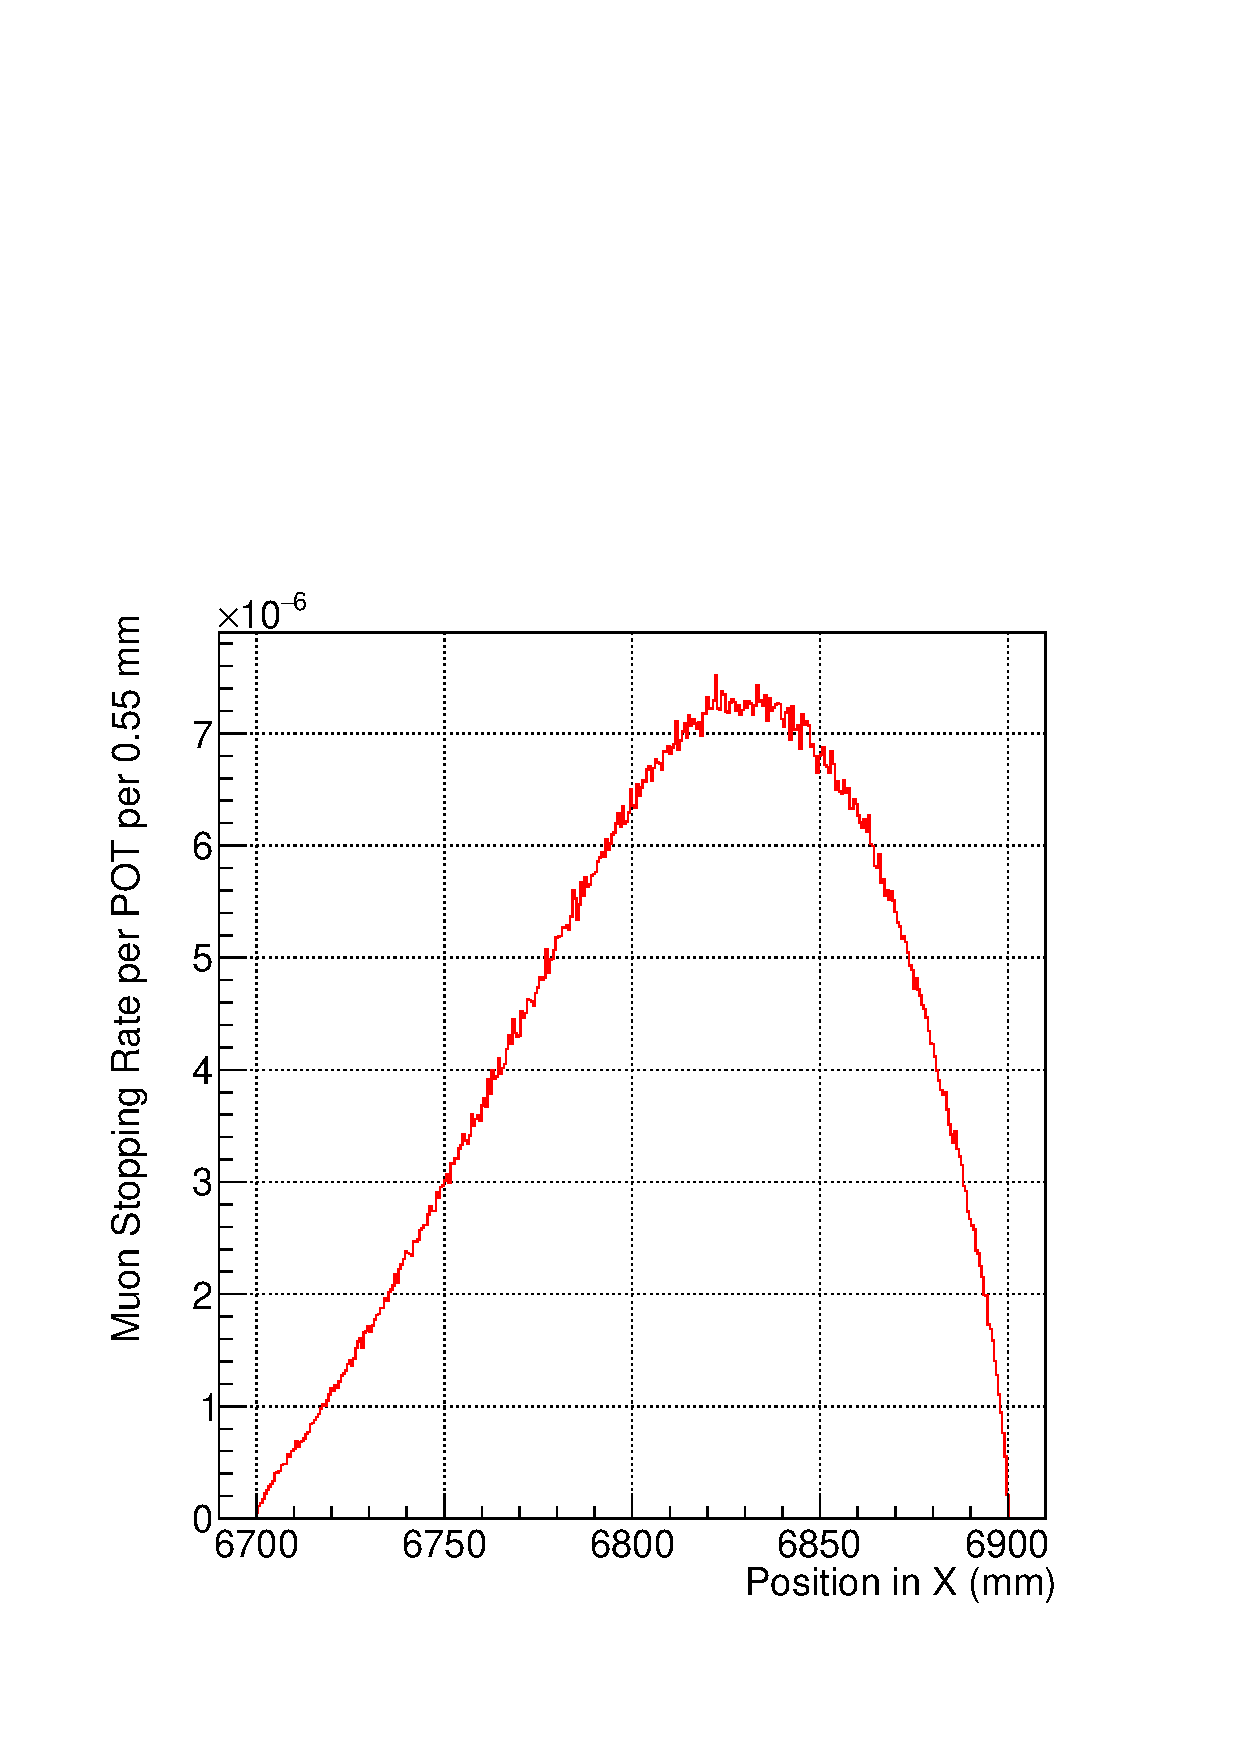
\includegraphics[width=0.33\textwidth,trim=0.3cm 1.5cm 0.7cm 1.2cm,clip]{figs/sensitivity/MuStops_1D_X.pdf}}
\subfloat[\figlabel{sense:stops:Y}Y axis]{
	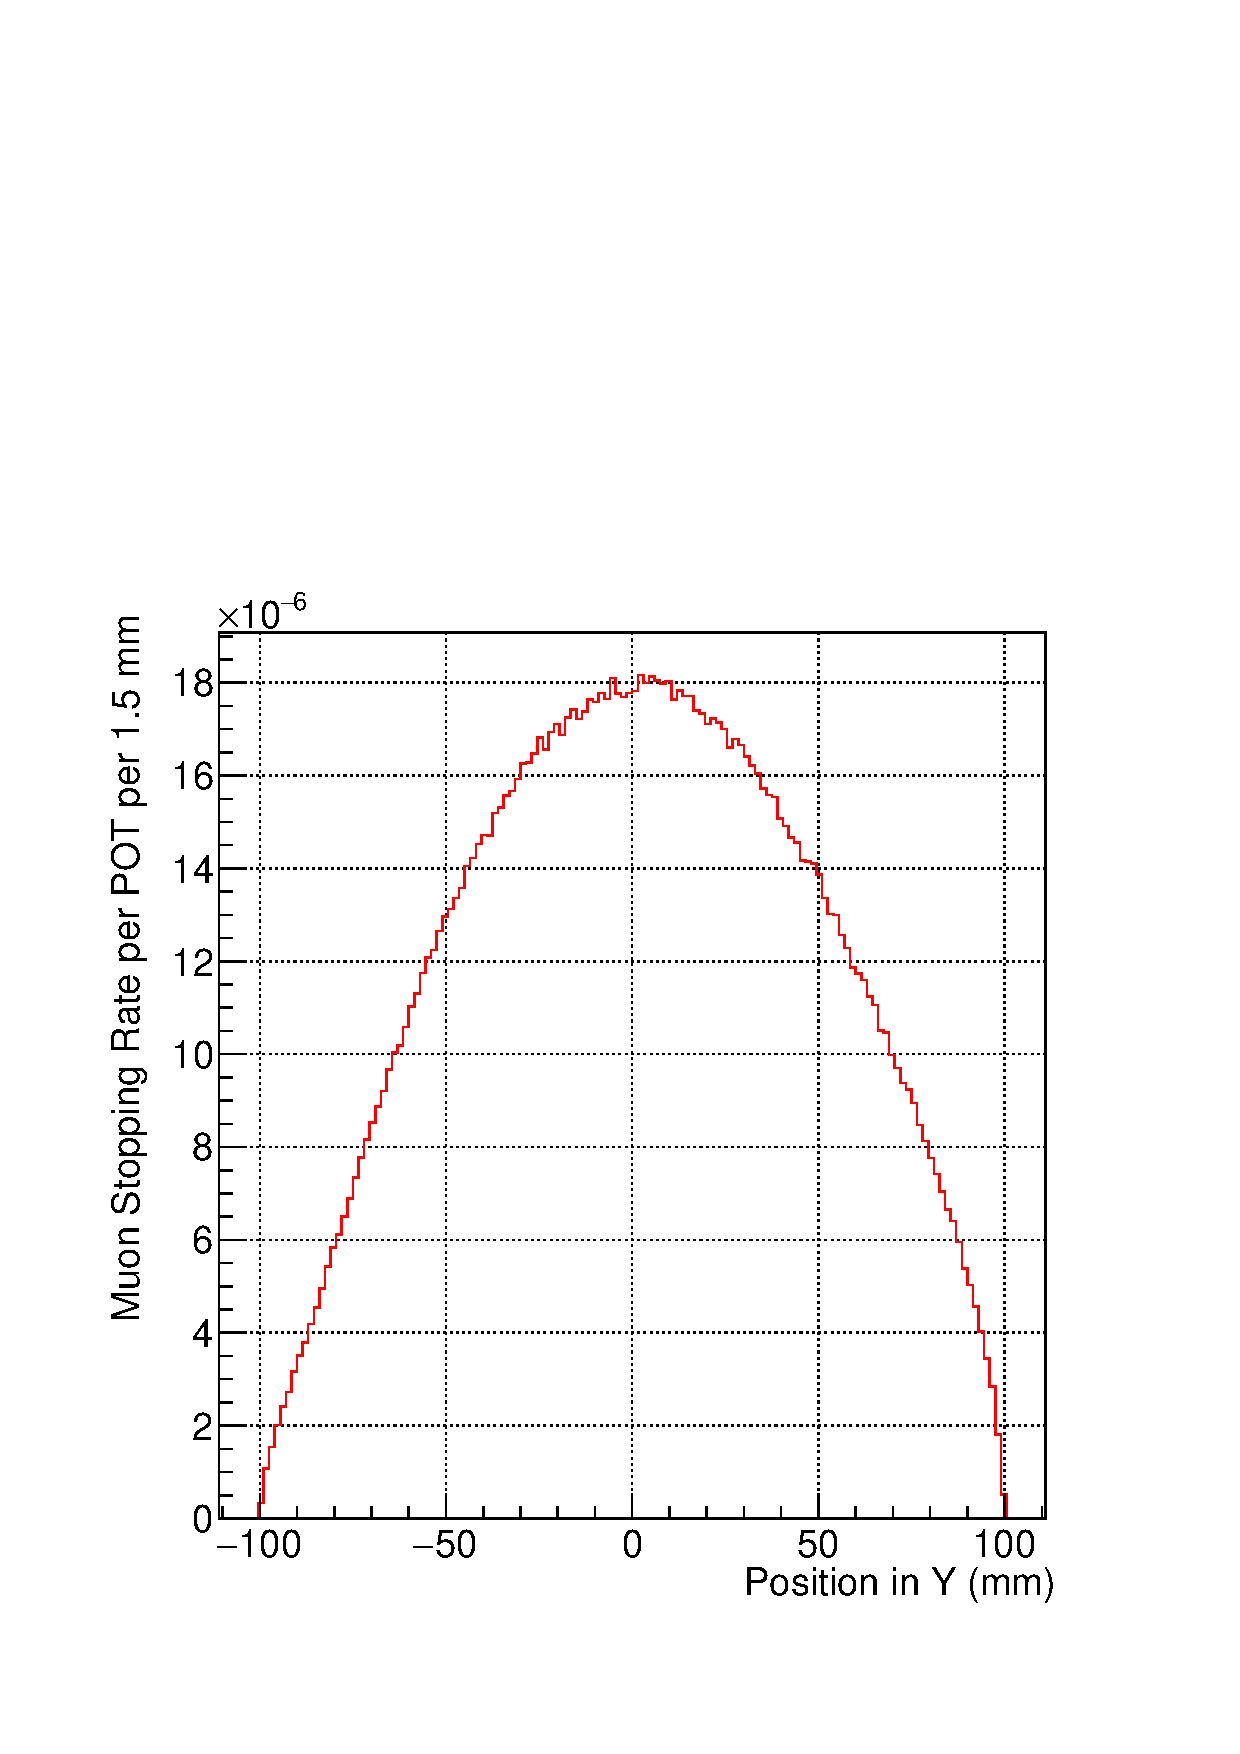
\includegraphics[width=0.33\textwidth,trim=0.3cm 1.5cm 0.7cm 1.2cm,clip]{figs/sensitivity/MuStops_1D_Y.pdf}}
\subfloat[\figlabel{sense:stops:Z}Z axis]{
        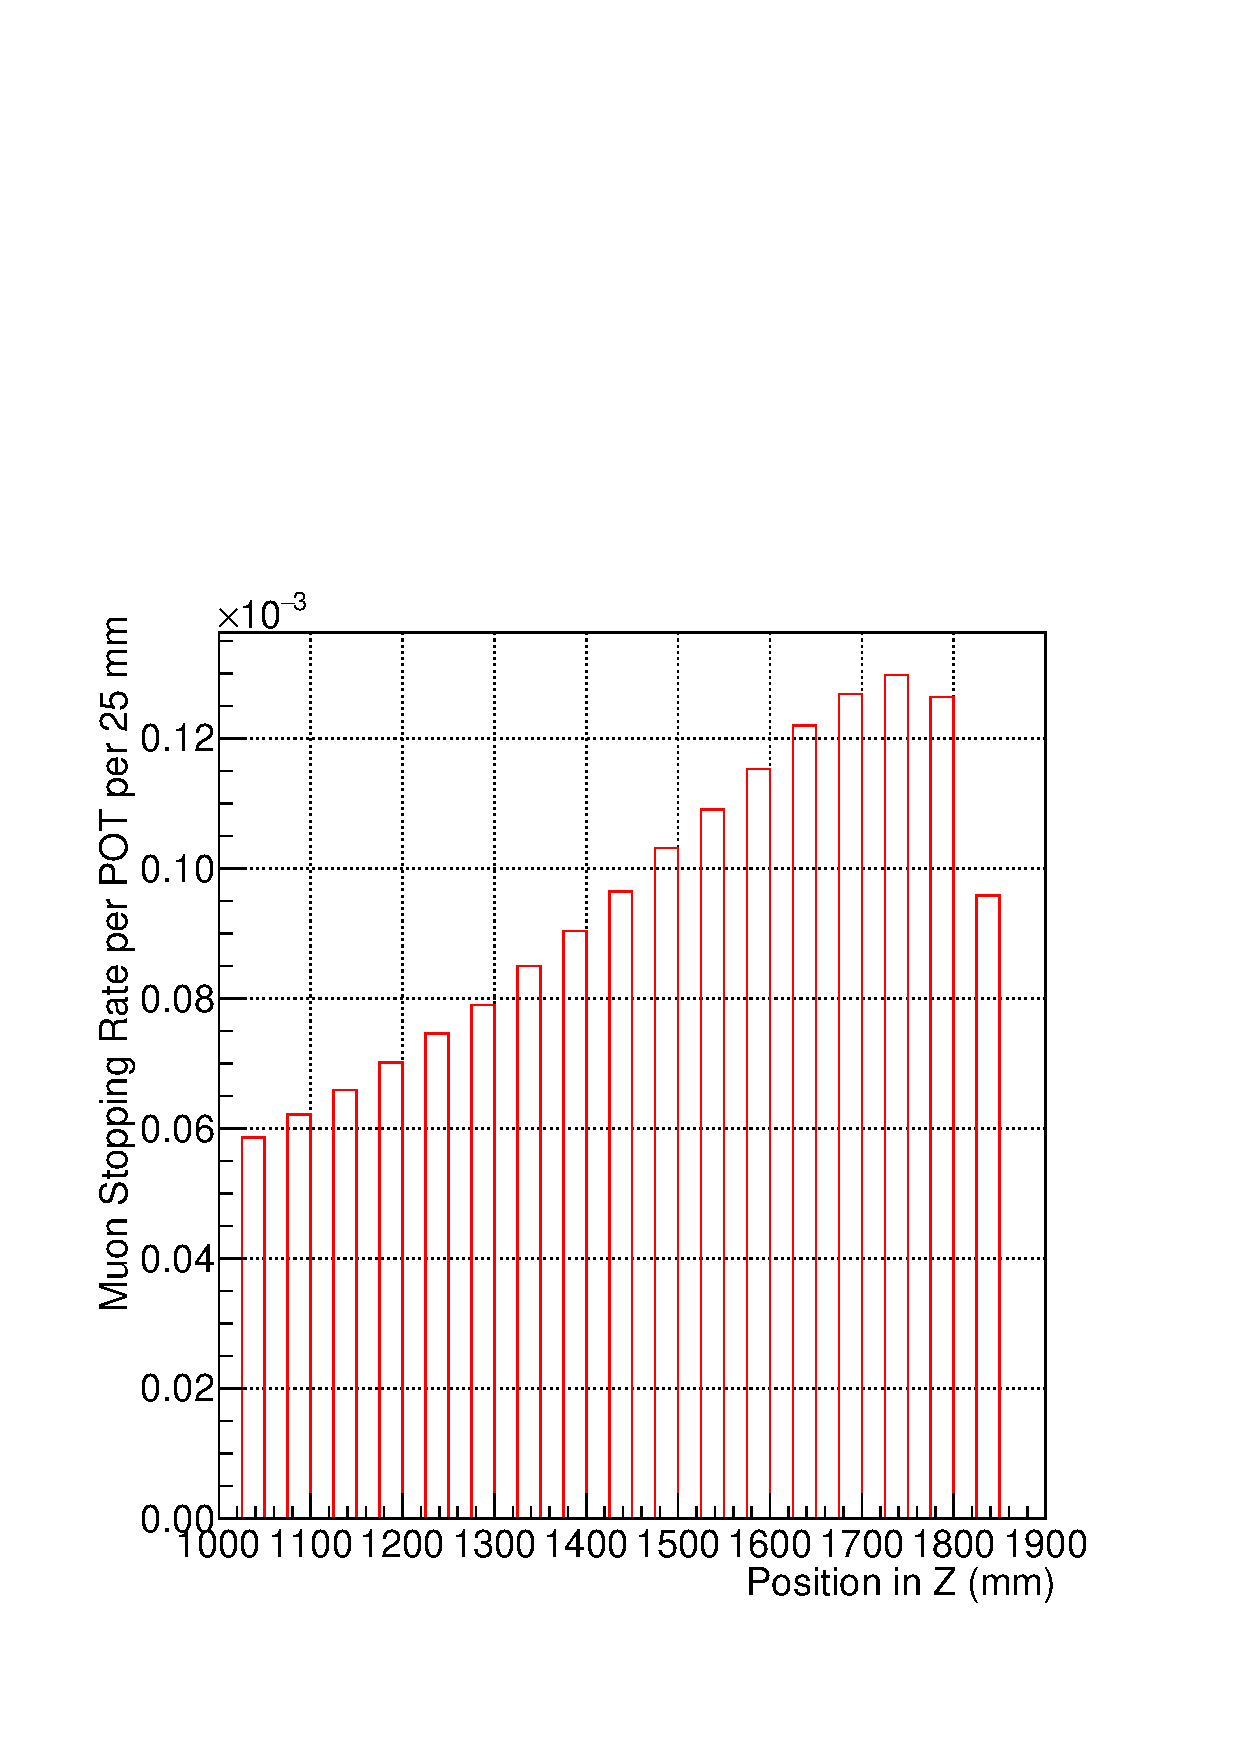
\includegraphics[width=0.33\textwidth,trim=0.3cm 1.5cm 0.7cm 1.2cm,clip]{figs/sensitivity/MuStops_1D_Z.pdf}}
\caption{\figlabel{sense:stops}
Projections of the final position of stopped muons in the stopping target.
	Axes are from the SimG4 global coordinate system, so that $+X$ points away from the production target, $+Y$ is vertically upwards, and $+Z$ is the direction of the muon beam at the production target.
	The muon beam in these plots is therefore travelling in the negative-$Z$ direction having passed around through 180\degree of the bent solenoid.
}
\end{figure}\xspace}

\newcommand{\FigSensGeomAccept}{%
\begin{figure}[bt]
\centering 
\subfloat[\figlabel{sense:accept:height}Path of Signal Electrons in the Beamline Projection]{
	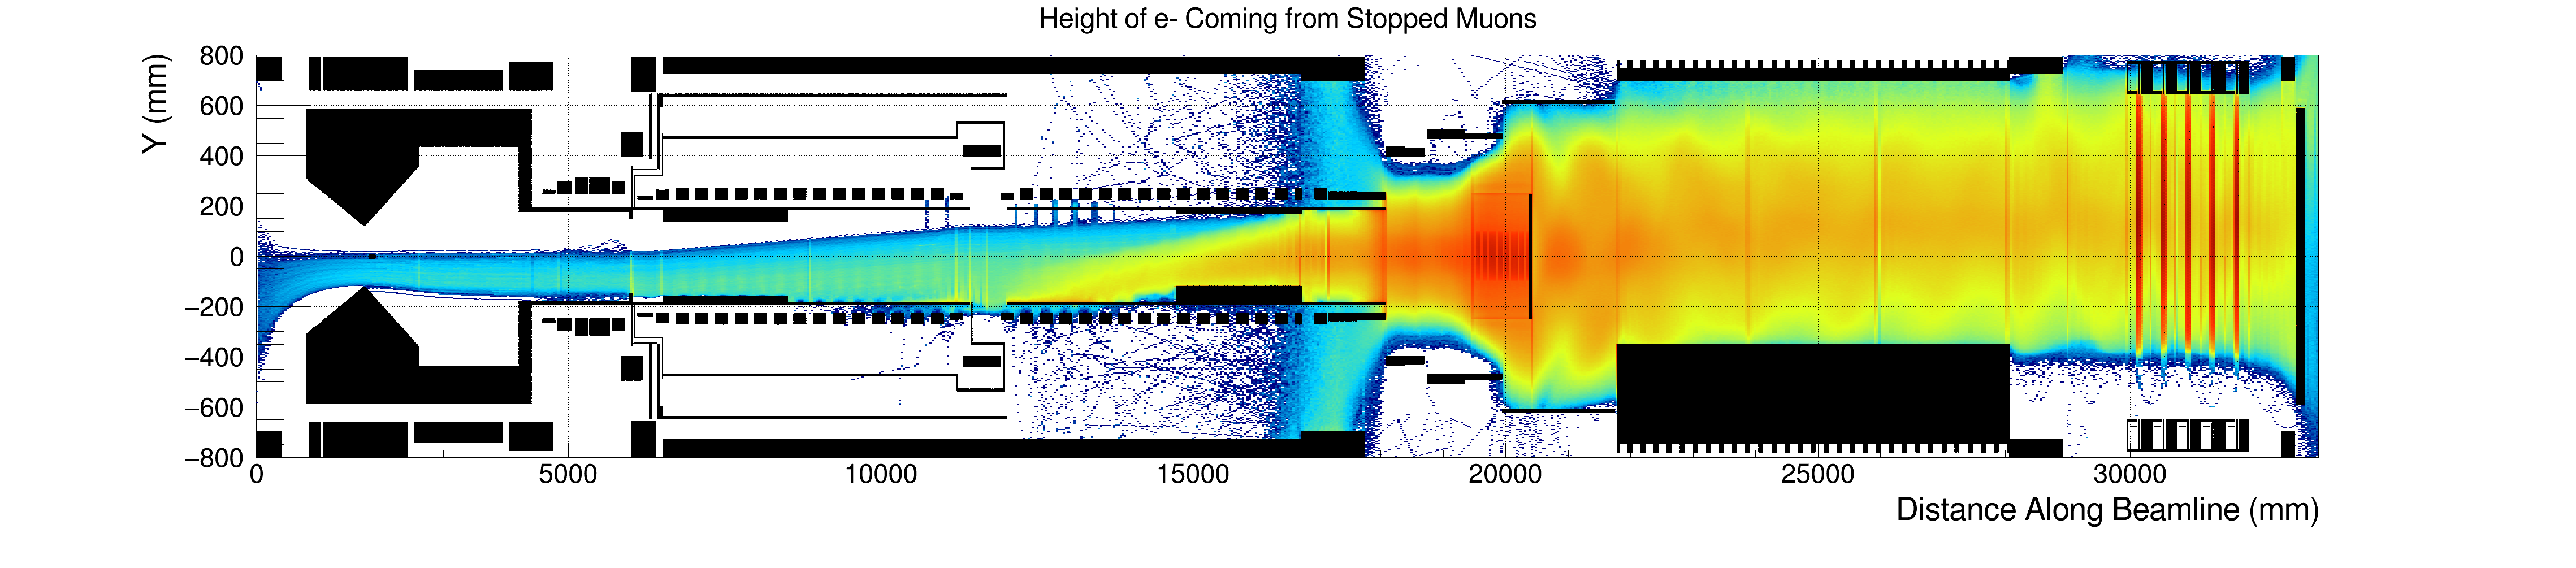
\includegraphics[width=0.99\textwidth,trim=8.3cm 1.5cm 13.2cm 2.2cm,clip]{figs/sensitivity/Tidied_SignalHeight2DVsBeamline.png}}\\
\subfloat[\figlabel{sense:accept:flux}Survival Probability for Signal Electrons]{
        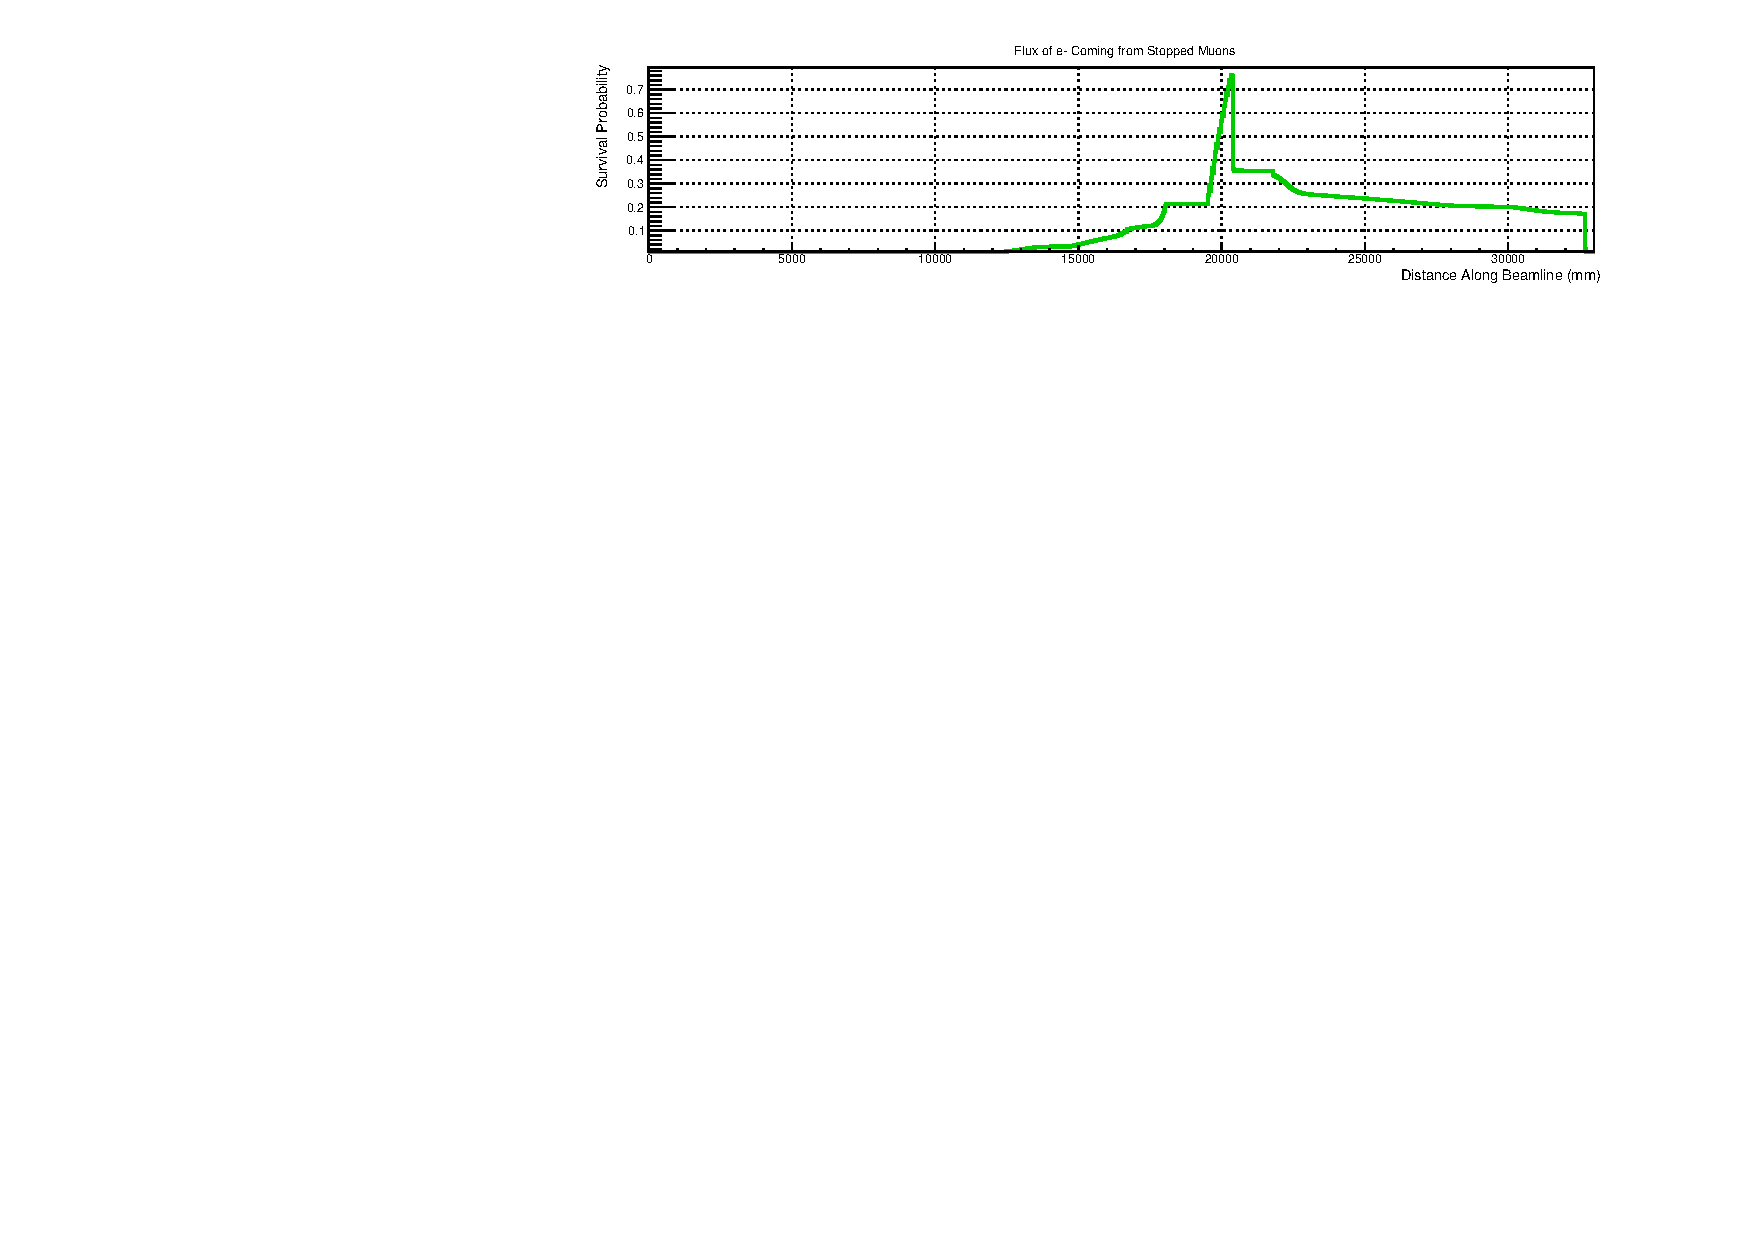
\includegraphics[width=0.99\textwidth,trim=1.0cm 0.2cm 1.7cm 0.4cm,clip]{figs/sensitivity/Tidied_SignalSurivivalVsBeamline.pdf}}
\caption{\figlabel{sense:accept}
Geometric acceptance of signal events.
\protect\subref{fig:sense:accept:height} Projection of the trajectories of signal electrons to the surface formed by the beamline axis and the vertical direction.
\protect\subref{fig:sense:accept:flux} Survival probability of signal electrons as a function of the distance along the beamline axis.
The x-axis range is the same in the two plots.
From these, it is clear how the acceptance is diminished by the DIO blocker in the spectrometer, although from that point on the rate of signal loss reduces.
}
\end{figure}\xspace}

\newcommand{\FigSensMomTransfer}{%
\begin{figure}[tb]
\centering 
%\fbox{
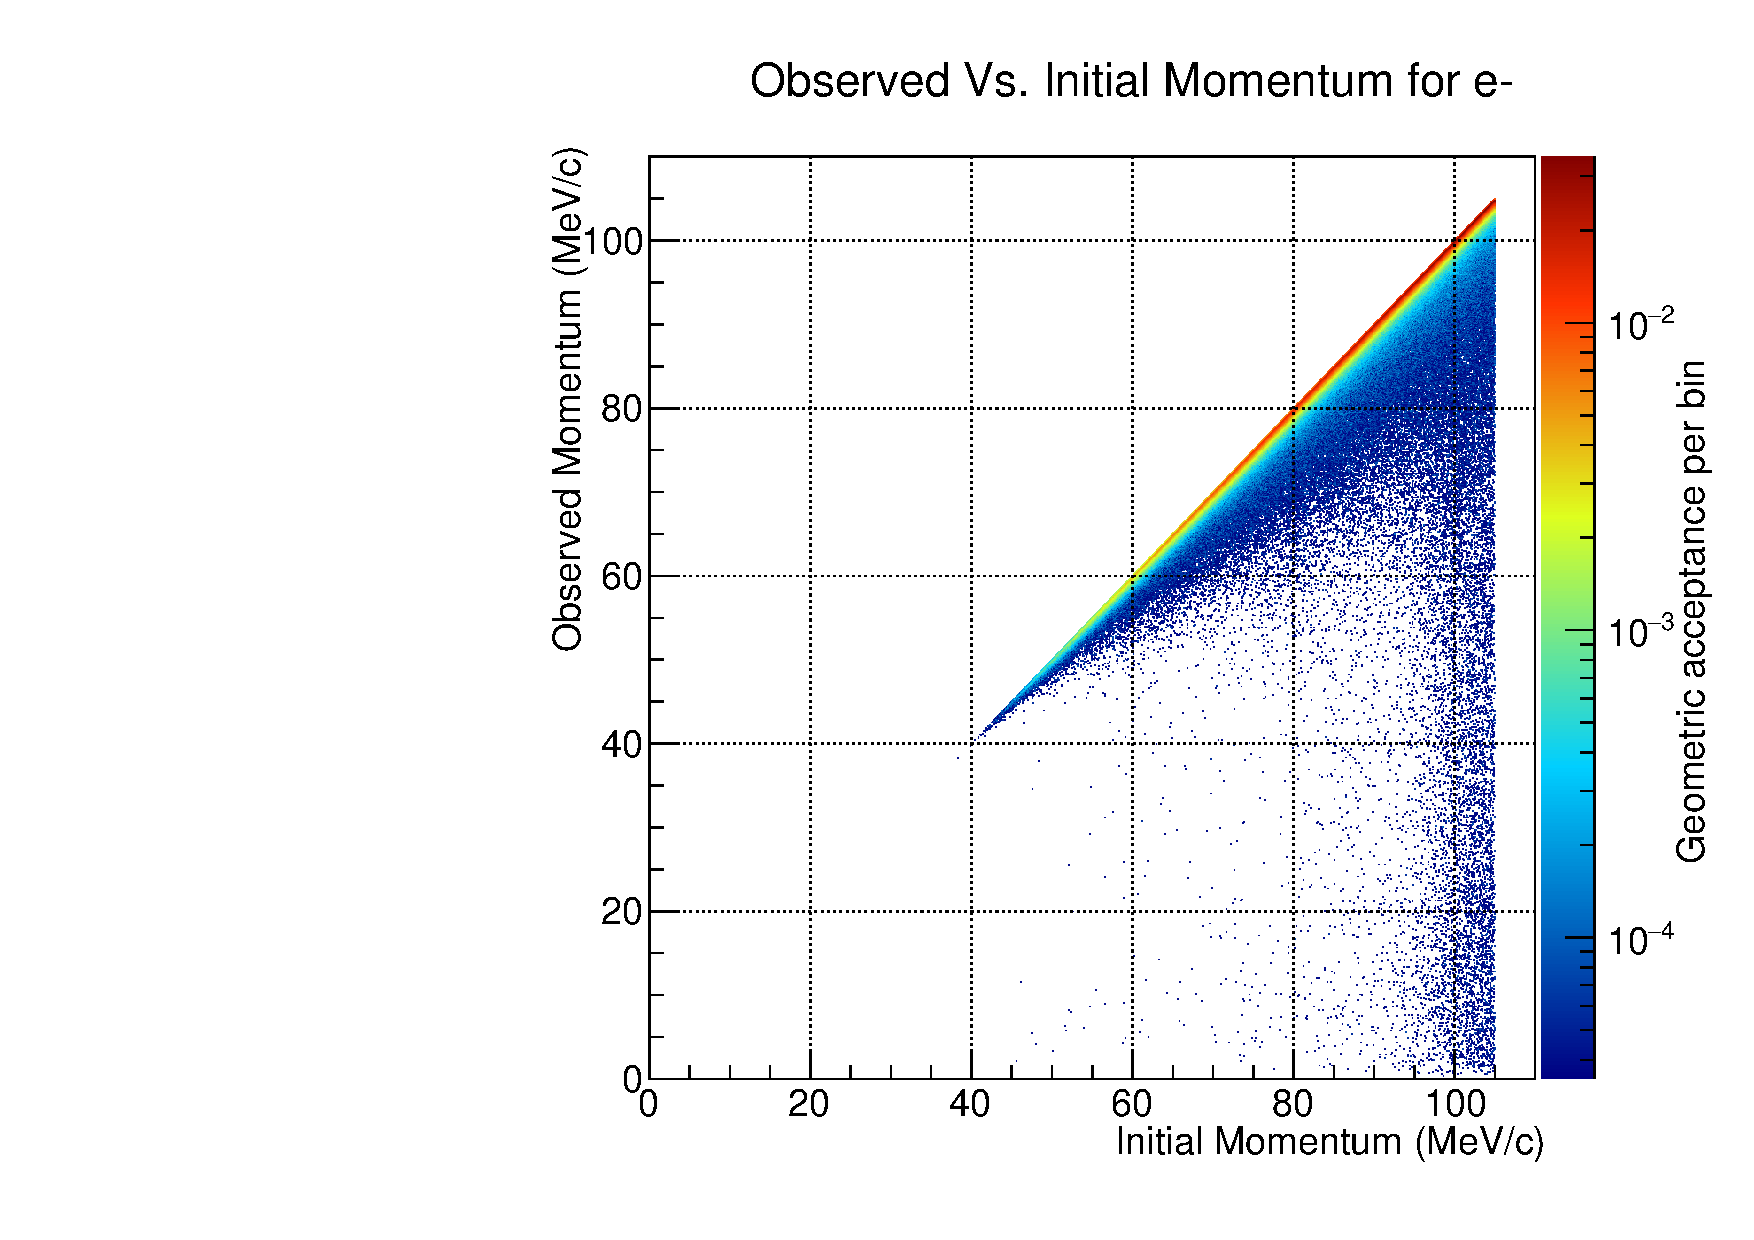
\includegraphics[width=0.5\textwidth,trim=0.0cm 0.0cm 0.0cm 1.6cm,clip]{figs/sensitivity/MomentumTransfer.pdf}
%}
\caption{\figlabel{sense:momTransfer}
The transfer matrix for electrons originating at the target, including the geometric acceptance and energy loss.
}
\end{figure}\xspace}

\newcommand{\FigSensMomSpectra}{%
\begin{figure}[tb]
\centering 
%\fbox{
\subfloat[Incl.~energy loss\figlabel{sense:spectra:ELoss}]             {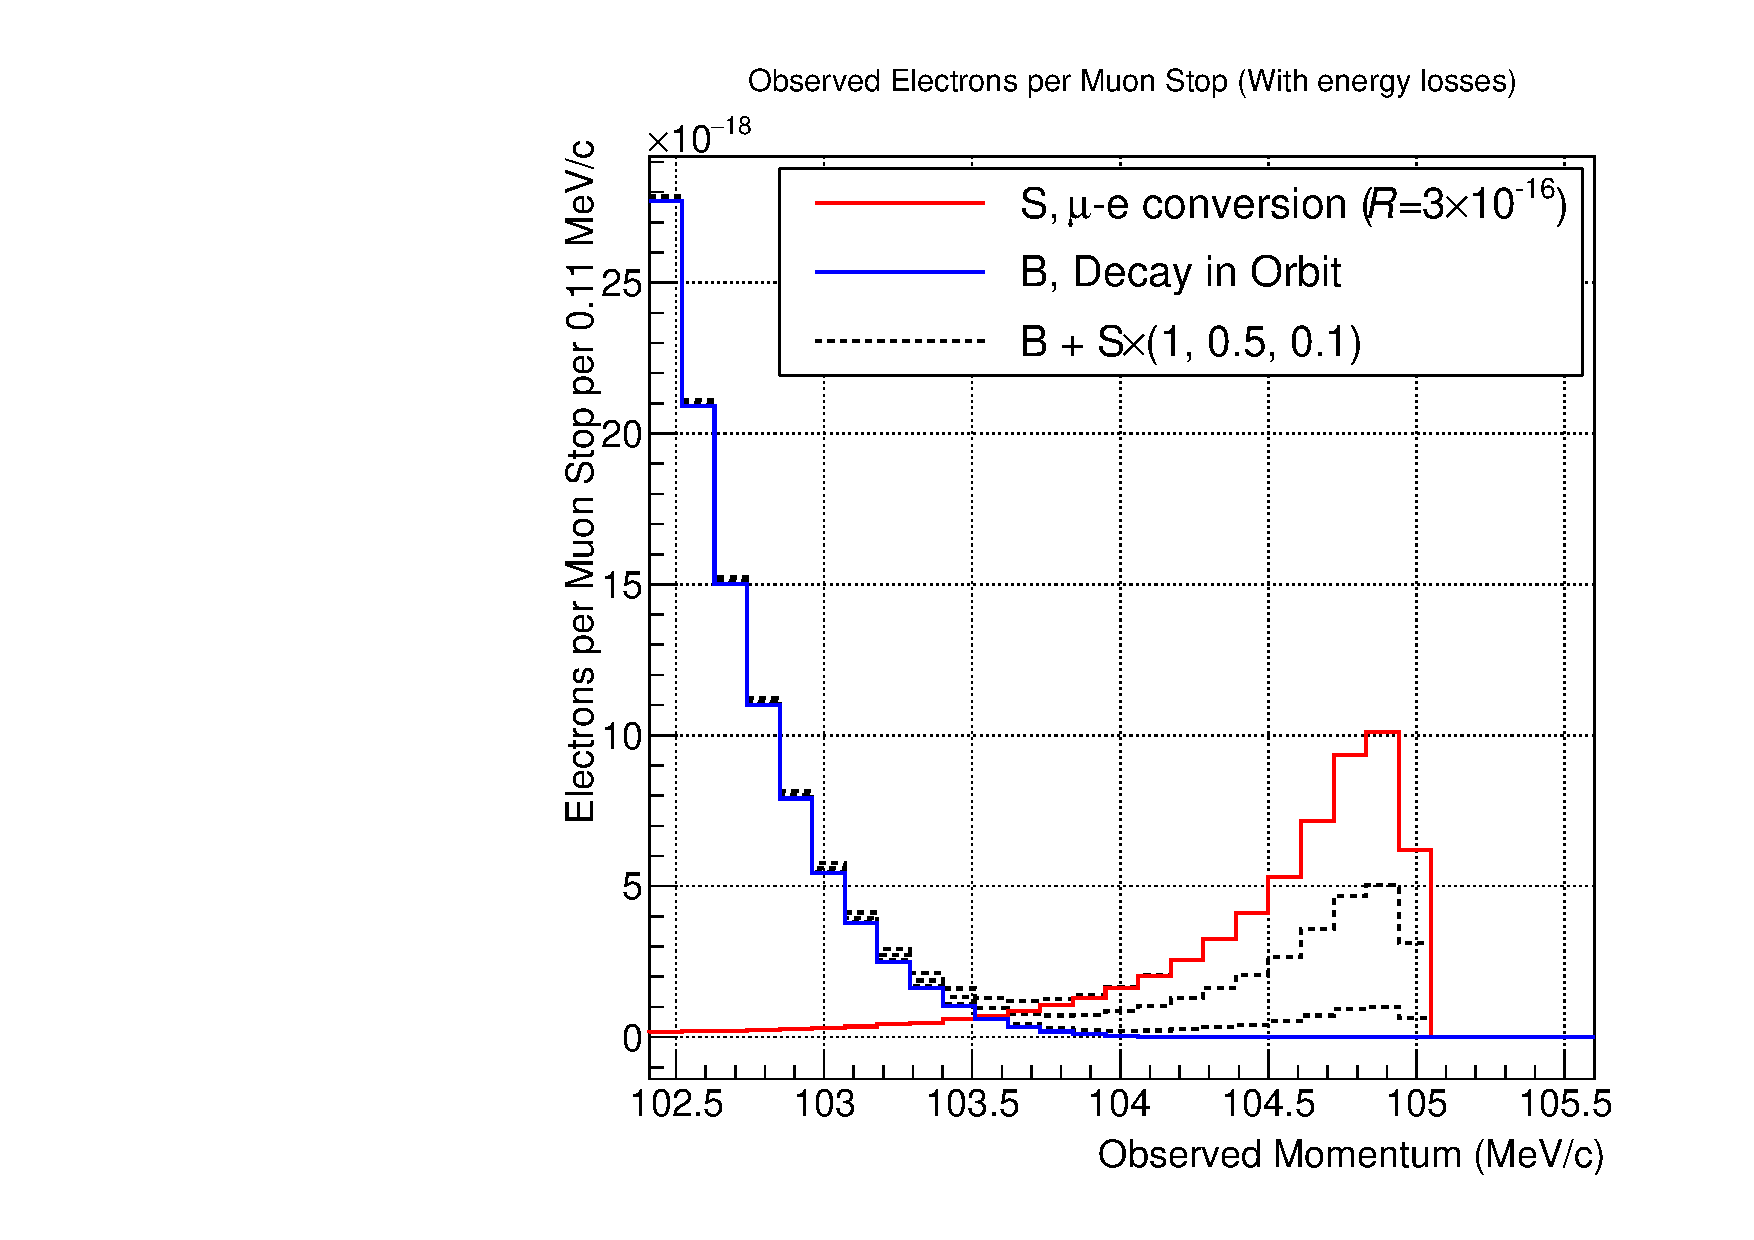
\includegraphics[width=0.48\textwidth,trim=0.0cm 0.0cm 1.0cm 1.0cm,clip]{figs/sensitivity/ConversionVsDio_Spectra.pdf}}
\subfloat[Energy loss \& resolution\figlabel{sense:spectra:resolution}]{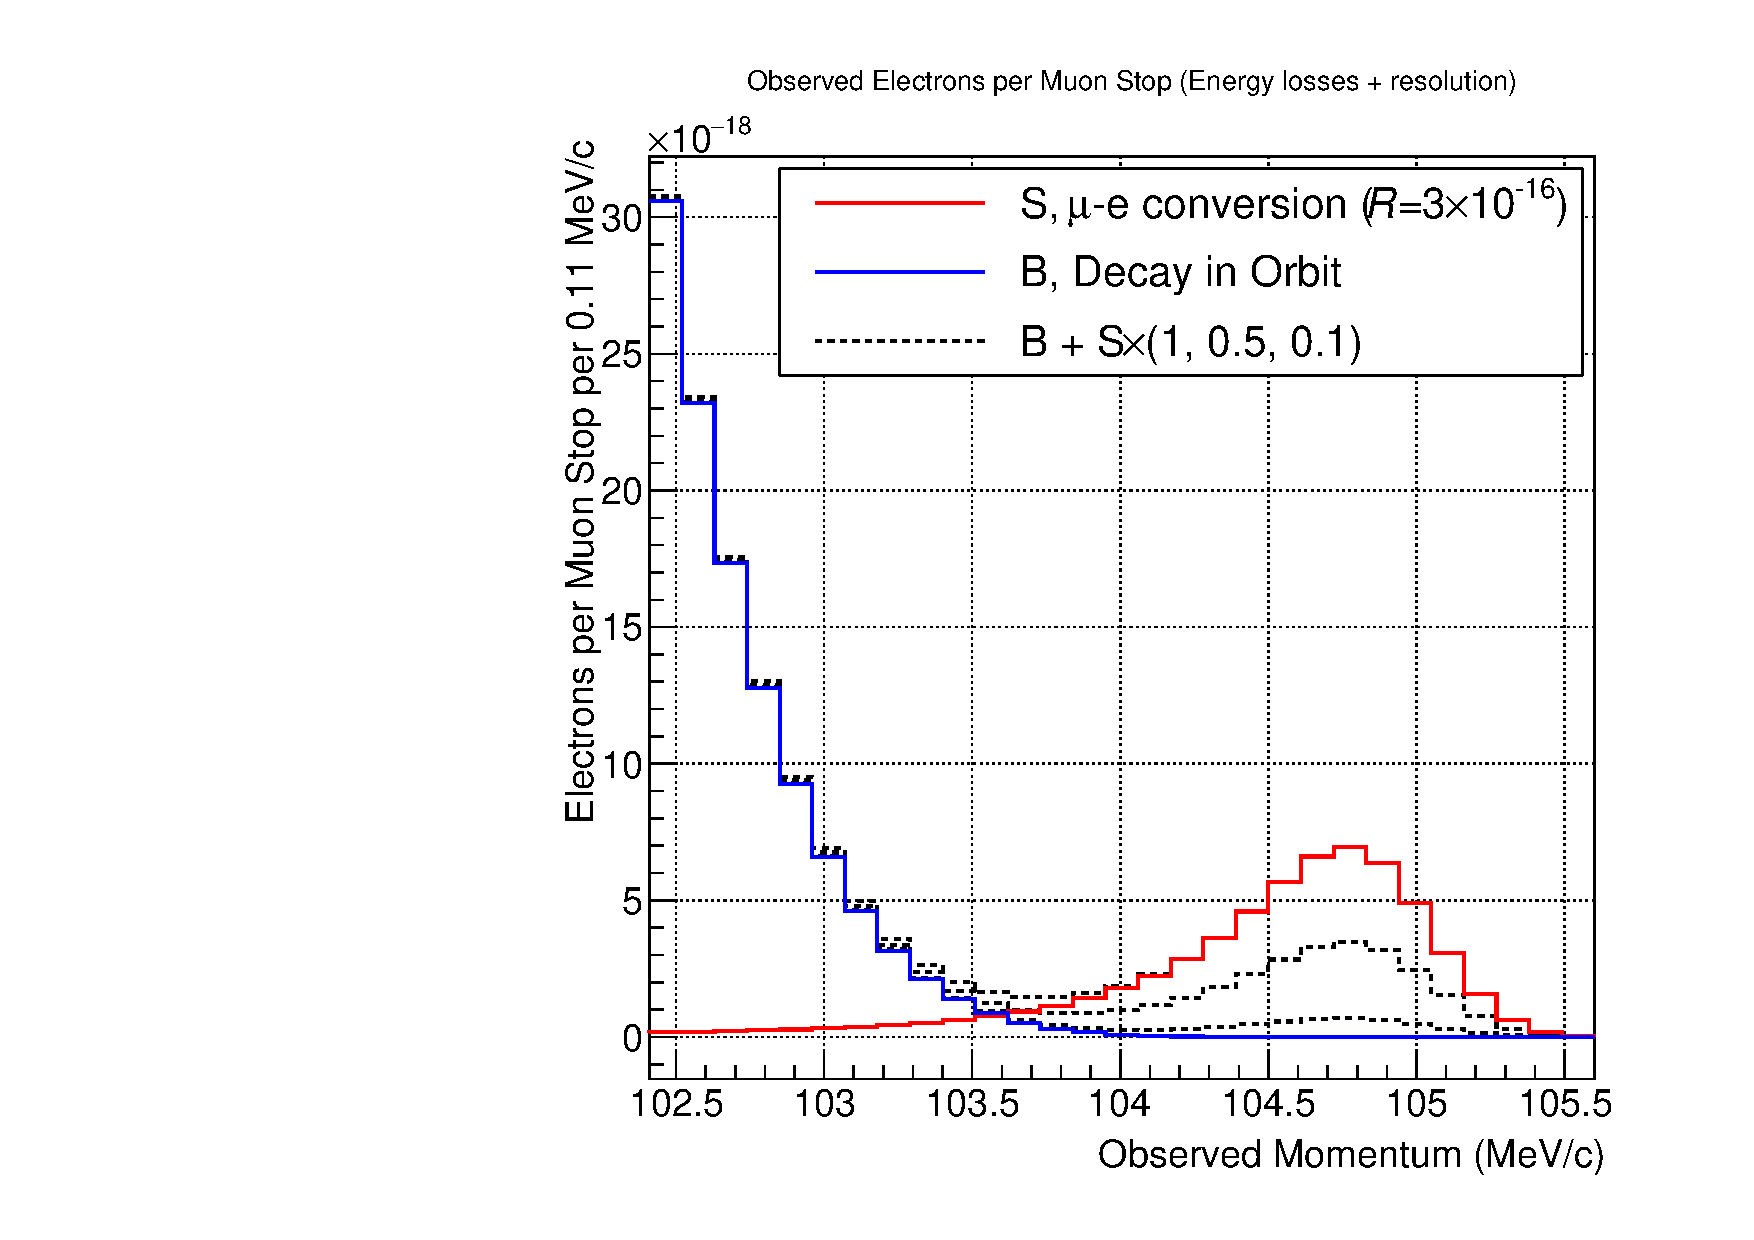
\includegraphics[width=0.48\textwidth,trim=0.0cm 0.0cm 1.0cm 1.0cm,clip]{figs/sensitivity/ConversionVsDio_Spectra-wResolution.pdf}}
\caption{
The spectrum of electrons coming from \ac{DIO} and \mueconv assuming a conversion rate of $\mathcal{R}=\sci{3}{-16}$.
Black dashed lines indicate the total electron distribution that would be seen (the sum of $S$ and $B$) if the signal has the assumed conversion rate of \num{3e-16}, half that rate, and one tenth that rate.
\protect\subref{fig:sense:spectra:ELoss} Includes energy losses in the target, beamline, and detector;
\protect\subref{fig:sense:spectra:resolution} also includes resolution effects (for a Gaussian resolution function with a standard deviation of $\sigma=200$~keV/c).
\figlabel{sense:spectra}}
\end{figure}\xspace}

\newcommand{\FigSensMomIntegral}{%
\begin{figure}[tb]
\centering 
%\fbox{
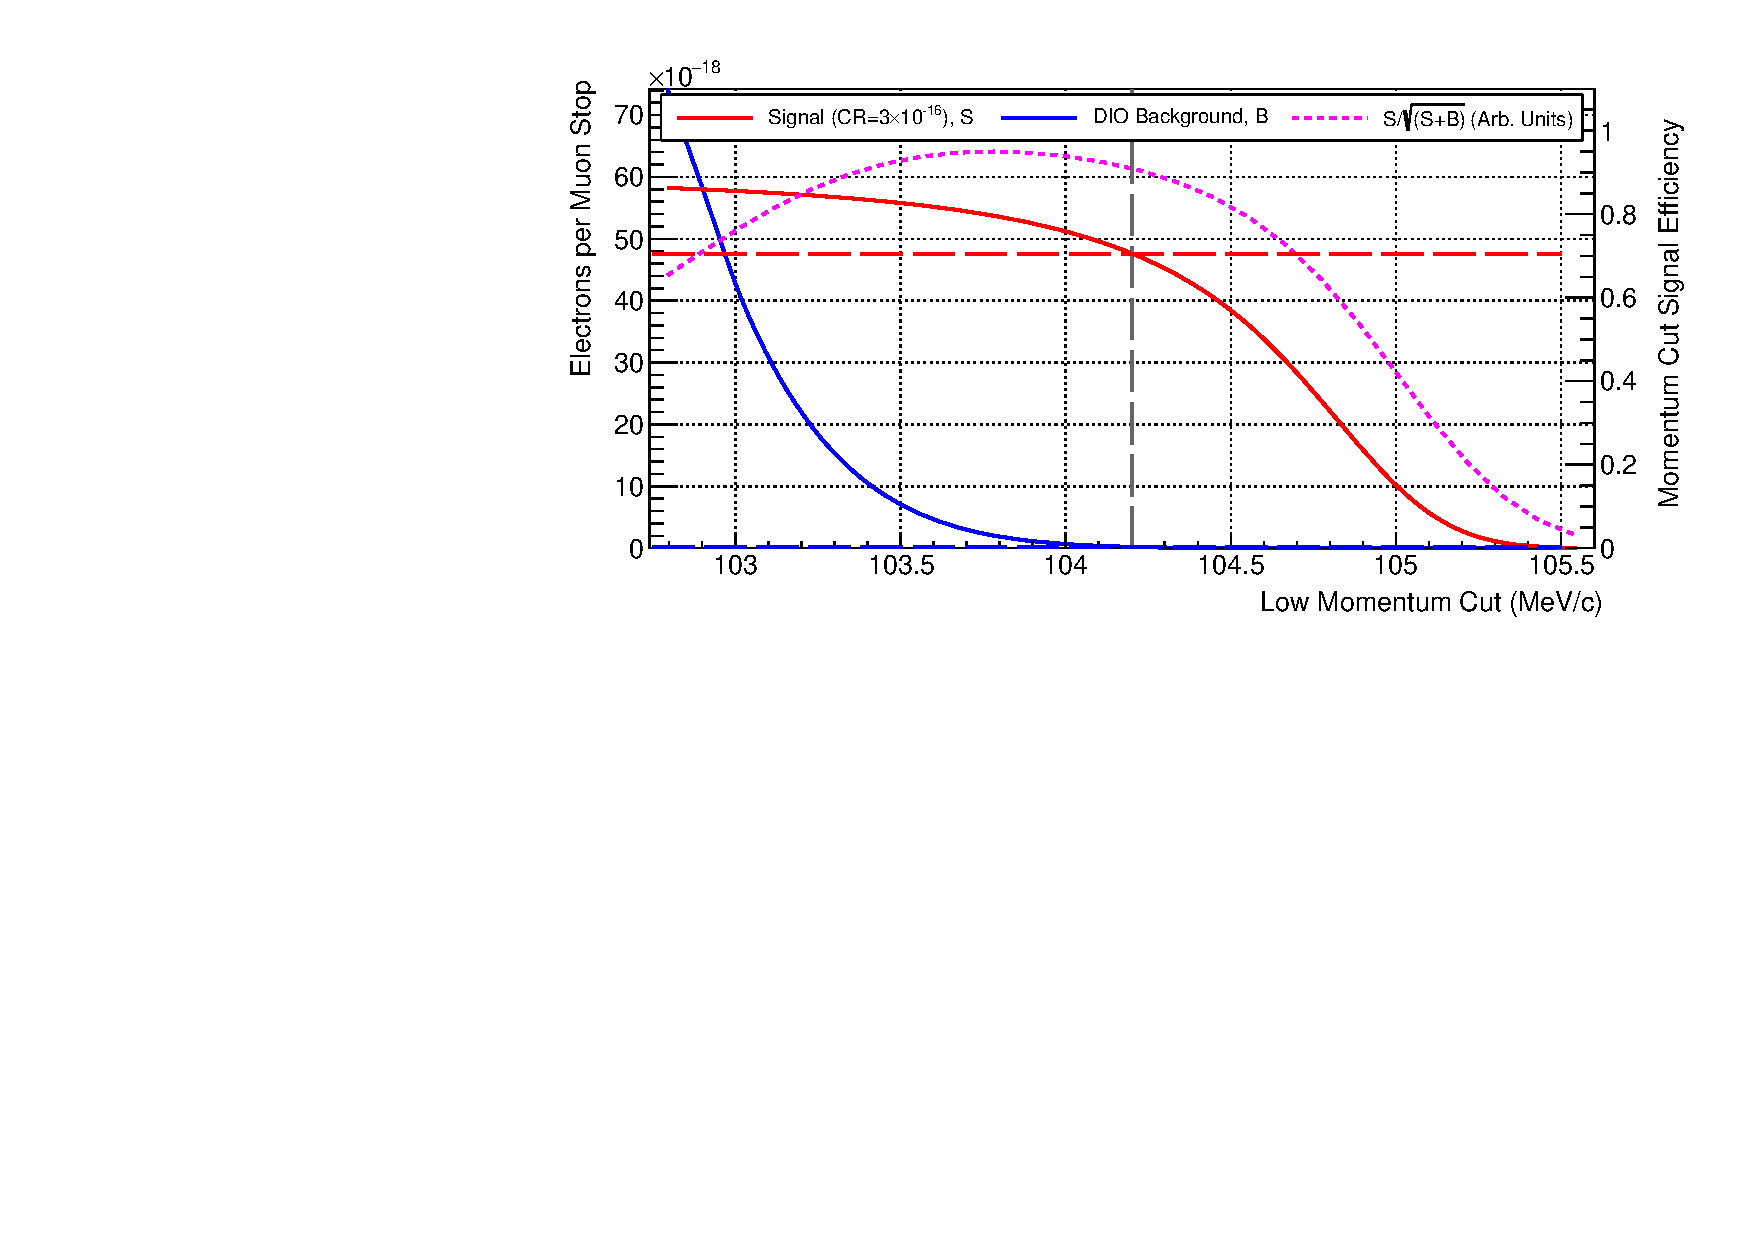
\includegraphics[width=0.99\textwidth,trim=0.5cm 0.0cm 0.5cm 0.3cm,clip]{figs/sensitivity/ConversionVsDio_Integrated.pdf}
%}
\caption{\figlabel{sense:integral}
Relative signal versus \ac{DIO} background as a function of the low-momentum cut value assuming a conversion rate of $\mathcal{R}=\sci{3}{-16}$.
The magenta line is the signal over square root of signal plus background for this conversion rate shown as an indicator of the optimum cut value.
}
\end{figure}\xspace}

\newcommand{\FigSensTiming}{%
\begin{figure}[b]
\centering 
%\fbox{
\subfloat[\figlabel{sense:timing:signal}Signal Arrival Time]      {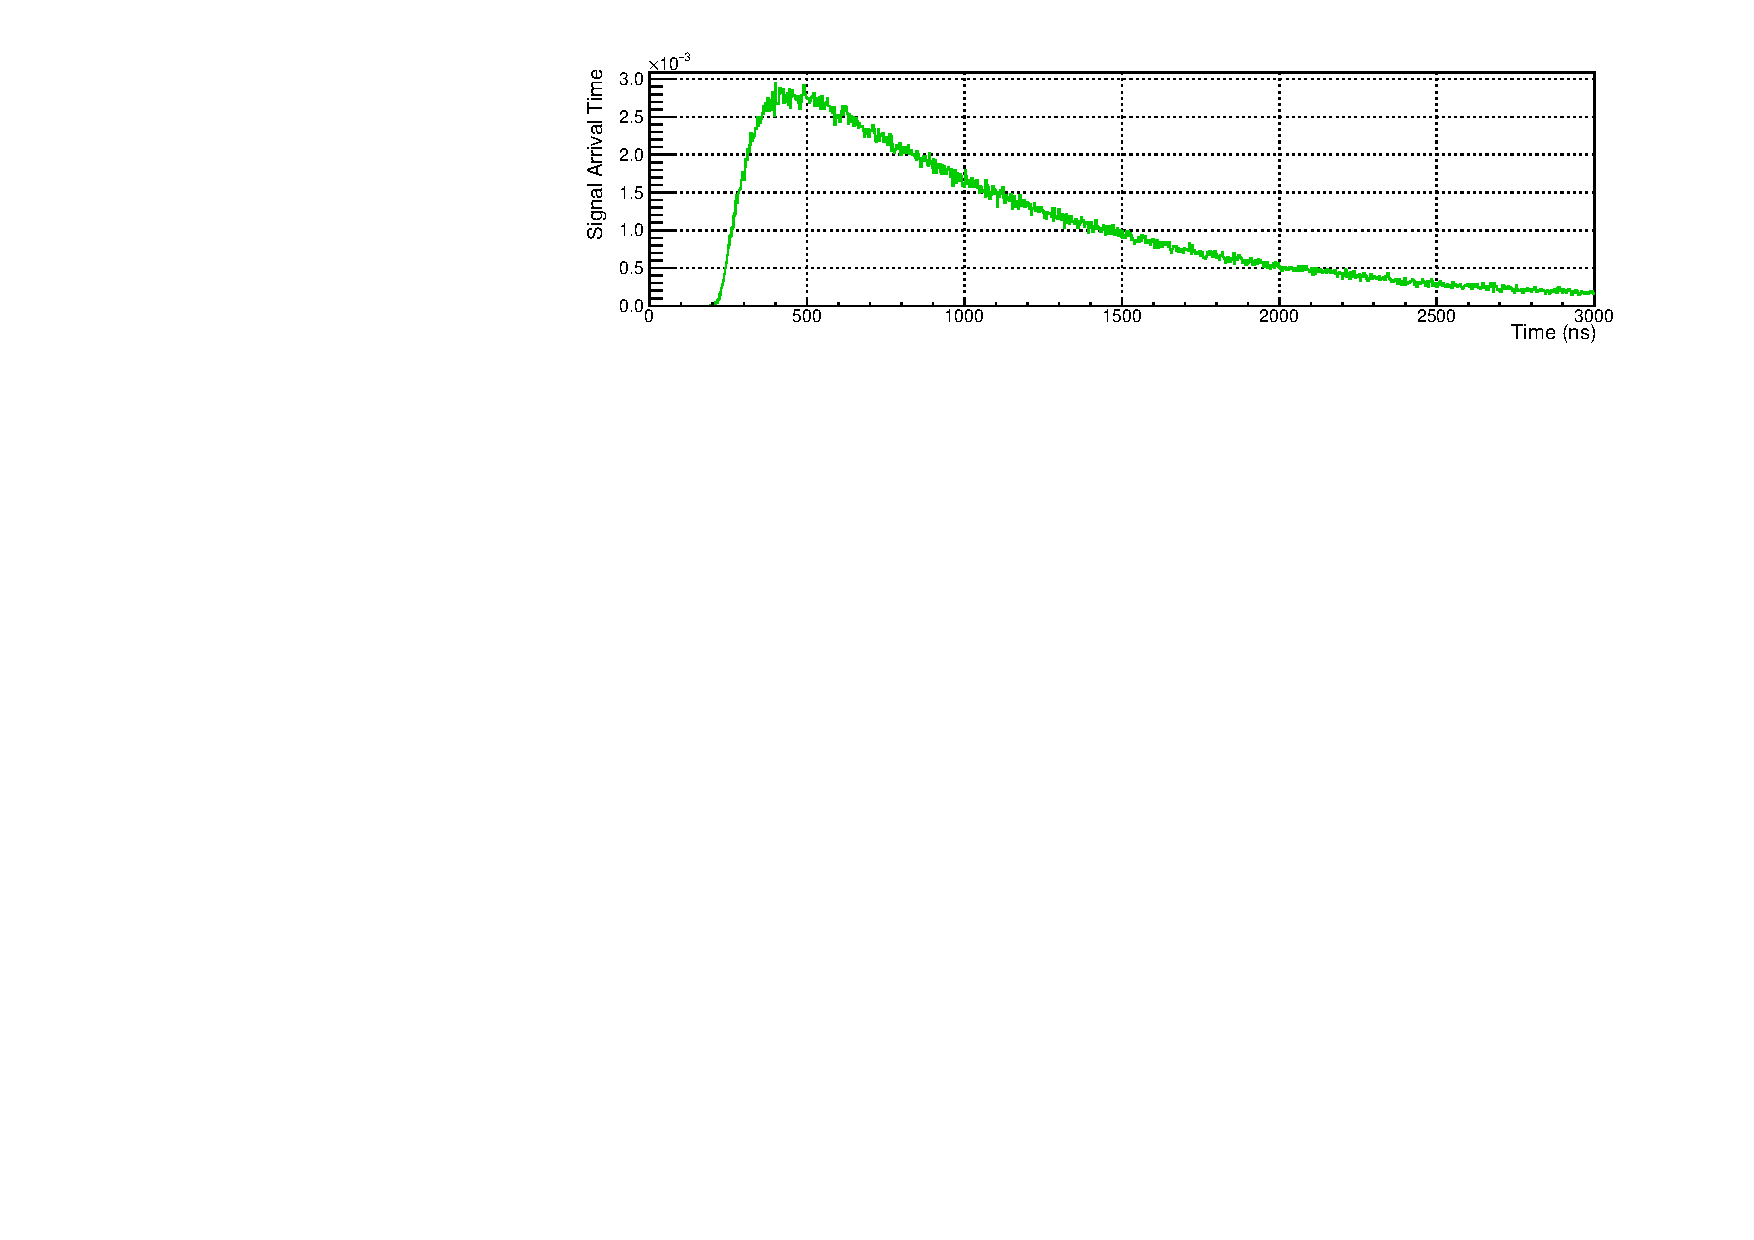
\includegraphics[width=0.9\textwidth,trim=0.9cm 0.1cm 1.5cm 0.20cm,clip]{figs/sensitivity/160823_MuonLifetime.pdf}}\\
\subfloat[\figlabel{sense:timing:efficiency}Timing Cut Efficiency]{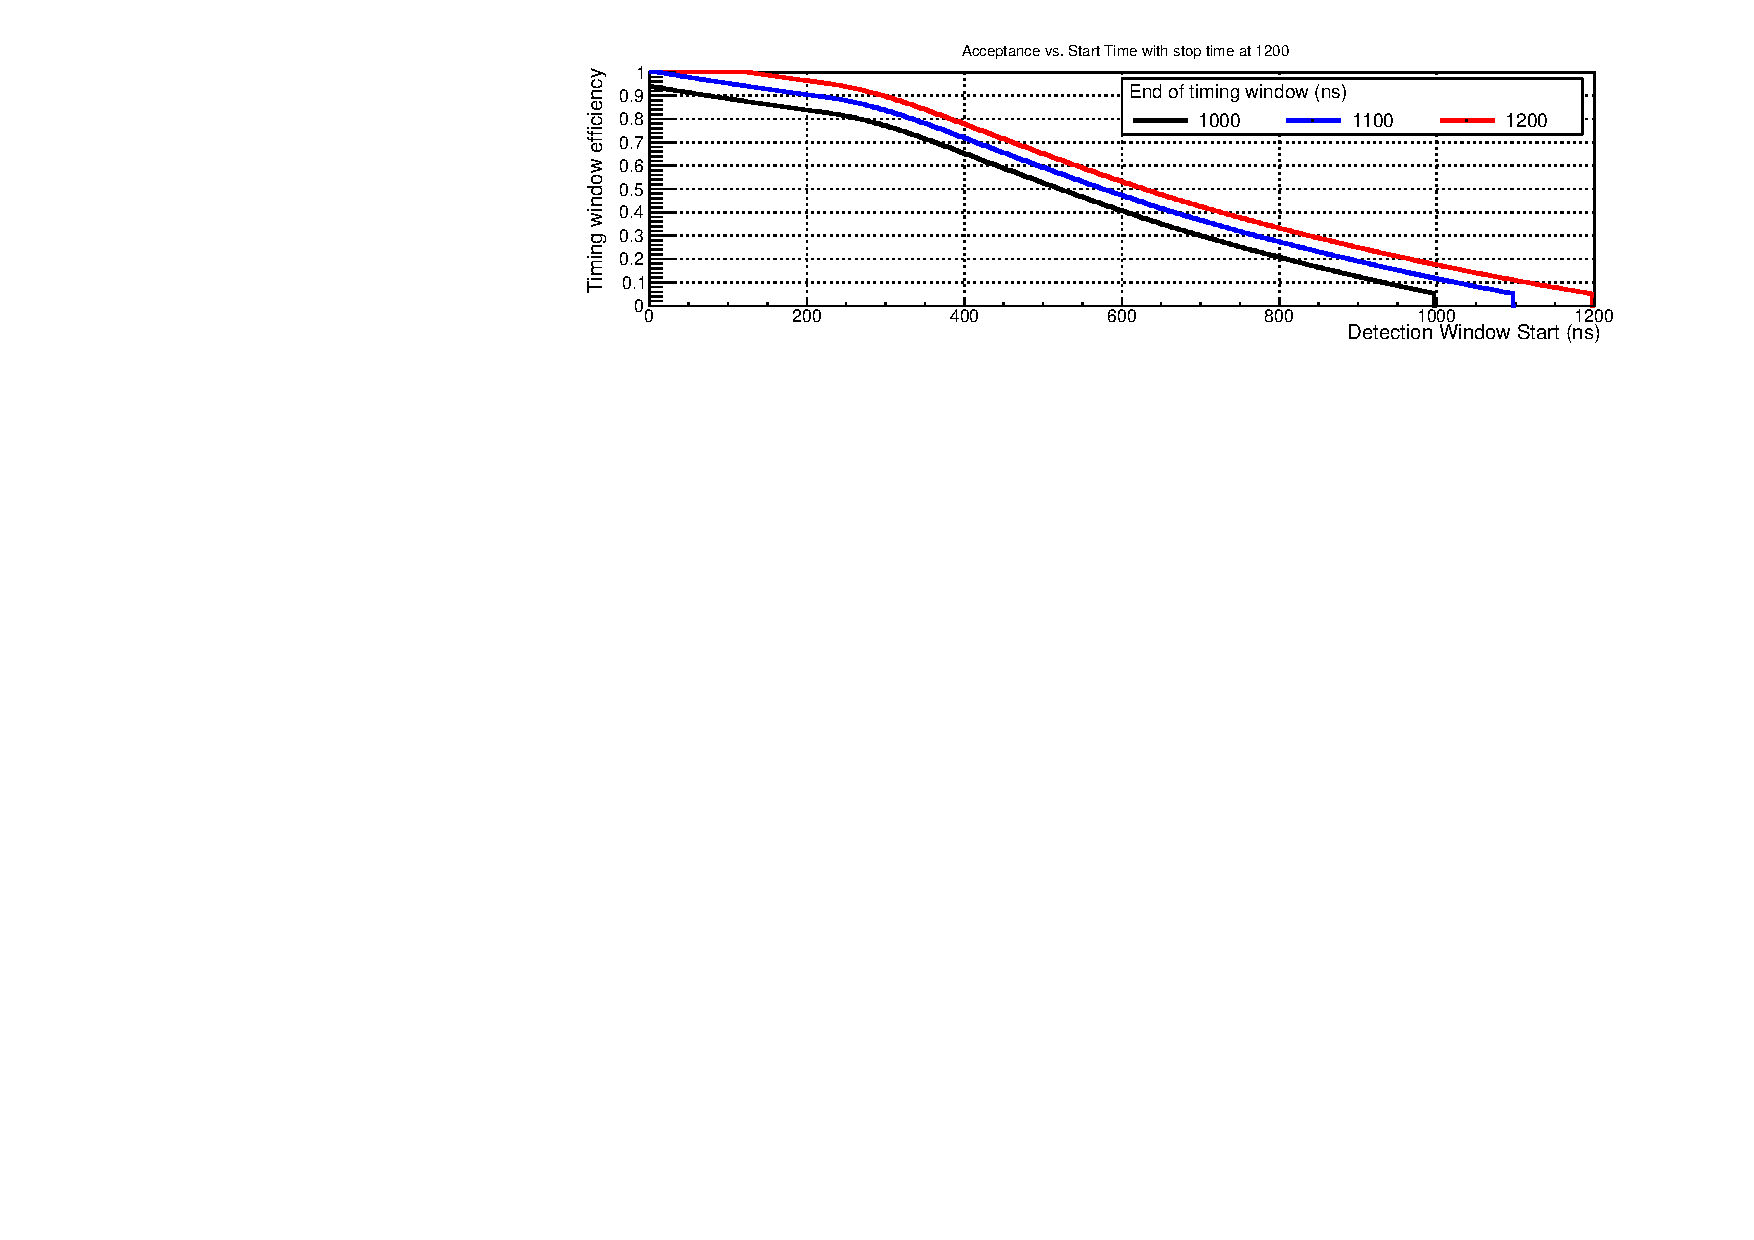
\includegraphics[width=0.9\textwidth,trim=0.9cm 0.1cm 1.5cm 0.4cm,clip]{figs/sensitivity/160823_TimingCutEfficiency.pdf}}
\caption{\figlabel{sense:timing}
Timing of signal electrons.
\protect\subref{fig:sense:timing:signal} The arrival time of signal electrons at the detector, including the effect of the proton pulse width, particle transportation, and the muon lifetime.
\protect\subref{fig:sense:timing:efficiency} the efficiency of the timing window as a function of the switch-on time.  Assumes a pulse separation of 1.17~$\mu$s.
}
\end{figure}\xspace}

\newcommand{\TabSensParams}{%
\begin{table}[b]
\centering
\begin{tabular}{lll}
	\hline
         $I_p$                          & 7~$\mu$A & Proton beam current                            \\ 
	 ${R}_{\mu/p}$      & \VarMuStopsPerPOT & Muon stopping rate per POT                     \\ 
%	 $f_\mathrm{1s}$                & 90\%    & Probability of reaching the ground state \\ 
	 $\mathcal{B}_\mathrm{capture}$ & 61\%    & Branching ratio for muon nuclear capture in Al \\ 
	 $A_{\mu\rightarrow e}$         & \VarTotalSignalAcceptance   & Total signal acceptance of \phaseII            \\ 
	\hline
\end{tabular}
        \caption{\tablabel{sense:ses}
        Parameters that determine the run time and single event sensitivity for COMET \phaseII based on this study.
        }
\end{table}\xspace}

\newcommand{\TabSensEstimates}{%
\begin{table}[t]
\centering
	\begin{tabular}{L{0.25\textwidth}p{0.14\textwidth}S[table-format=2.1]p{0.12\textwidth}p{0.23\textwidth}}
	\hline
							& Single event sensitivity & \multicolumn{1}{p{0.13\textwidth}}{Total \acp{POT} ($\times10^{19}$)} &Beam time $t_\textrm{run}$ (s) & SES in one year of continuous beam \\ 
  \hline
  COMET \phaseII\hspace{1ex}(this study)                & \VarPredictedSES         & 68.3 & \VarRunTime[3]                  & \VarPredictedSESPerYear                         \\ 
  COMET \phaseII\hspace{1ex}(CDR 2009~\cite{CDRphase2}) & \sci{2.6}{-17}           & 85   & \sci{2.00}{7}                  & \sci{1.65}{-17}                         \\ 
  Mu2e~\cite{Mu2e2014}                                  & \sci{2.4}{-17}           & 36   & \sci{6.00}{7}                  & \sci{4.57}{-17}                         \\ 
  COMET \phaseI~\cite{TDR2016}                          & \sci{3.0}{-15}           & 3.2 & \sci{1.26}{7}                  & \sci{1.19}{-15}                         \\ 
	\hline
\end{tabular}
        \caption{\tablabel{sense:comparisons}
        Comparison between the run time and single-event sensitivity from this study and from the 2009 CDR, the \phaseI TDR, and  the Mu2e experiment's TDR.
	The \ac{ses} in one year of continuous beam is the single-event-sensitivity that can be achieved in \num{3.15e7}~seconds of running, assuming no beam shutdown periods.
        }
\end{table}\xspace}

\chapter{COMET \phaseII: Signal Sensitivity}
\sectlabel{sense}
As discussed previously, the signal sensitivity of COMET is a measure of the ability both to produce a signal event
and to detect it.
The signal efficiency per \ac{POT} is therefore the product of the muon stopping rate, the rate of muon capture from the ground state of a muonic atom (the normalisation in the conversion rate), and the total signal acceptance after all analysis cuts and geometric acceptances are considered.
%This product is analogous to the cross section times branching ration often used to describe collider efficiencies.

Since signal efficiency describes only the ability to produce and detect signal, this chapter could in principle ignore all possible backgrounds.
However in order to tune analysis cuts, one must consider the potential background rates at some level, which must be minimised and controlled.
Until the full analysis chain is implemented, we consider only a handful of crude analysis cuts, namely the momentum and timing of electrons.
The 2009 \ac{CDR} additionally included cuts on the reconstruction~\cite{CDRphase2} such as track fitting quality, and the ratio between transverse and longitudinal momentum of particles (related to the pitch angle).

\FigSensMuMomentum
\section{Muon Stopping Rate}
\sectlabel{sense:stops}
%\begin{easylist}
%# 1.64e-3 per POT
%# Comparison of muon momenta: before collimator, around target, stopping in target, passing beam blocker
%# Profile in target
%# Timing of muon stops
%# Asymmetry in X
%# Y dependence due to momentum dispersion
%# Scope for improvements, see appendix
%# Effect of proton beam
%# Hadron production model?
%\end{easylist}
Based on a simulation of some 1.1 billion \acp{POT}, the muon stopping rate of the optimised design was found to be \sci{1.61}{-3}~per \ac{POT}.
This amounts to 43\% of the muons that reach the target itself, a fraction that is determined mostly by the muon momentum distribution and the total amount of target material, as demonstrated by \fig{sense:muMomenta}
showing the momentum of muons at different points in the beam.

\Fig{sense:stops} shows where muons stop in the target based on this simulation from which it is clear that several asymmetries and correlations exist.
For example, the correlation between Z and Y shown in \fig{sense:stops:ZY} arises due to the dispersion in the muon beam when it arrives at the target. 
Since high-momentum muons are vertically lower (towards negative Y) in the beam, and since these muons have a larger stopping distance, muons lower down in Y tend to travel further through the target (towards lower values of Z).
It is interesting, however, that when the integration is taken over all target disks the distribution in Y demonstrates little asymmetry (\fig{sense:stops:Y}). 
This is most likely due to the fact that the Y-position is controlled by the Torus1 and Torus2 dipole fields which were optimised to maximise the stopping rate, which one might expect to be achieved when the stopping distribution is symmetric.

\FigSensMuStopsTwoD
Given this correlation, there might be a gain in signal sensitivity if there were less material at the top of the target.
Since this material is less important for stopping the low-energy muons, removing the extra material might have little impact on the stopping efficiency.
On the other hand, it will likely increase signal acceptance since signal electrons will pass through less material.

Whilst the vertical stopping distribution is largely symmetric,
a striking asymmetry exists in the horizontal stopping distribution (\fig{sense:stops:X}).
The cause of this asymmetry is unclear at this stage.
It could arise from the fact that the production target itself is asymmetric in the horizontal transverse direction, such that more muons and pions are produced to one side of the beam axis.
On the other hand, it could also arise from the transportation dynamics of the bent solenoid, dipole field and collimator design. 
Since this asymmetry could suggest low-energy muons are missing the target on one side, studying the cause of this asymmetry 
is an important avenue to pursue for further gains in \ac{SES}.
%is important as removing it could be another source of sensitivity increase.
%Both of these possibilities should be studied further in the future as a potential method for increasing the muon stopping rate.

%Further increases in the stopping rate might be achieved by adding additional 

\section{Acceptance of Stopping Target Electrons}
\FigSensGeomAccept
%\begin{easylist}
%# Geometric acceptance
%## Flux plot and beamline height plot
%# Momentum transfer matrix
%# Momentum cut efficiency
%## Spectrum after energy loss
%## Spectrum after realistic resolution (TODO)
%## Integrate downwards plot, with $S/\sqrt(S+B)$
%# Timing cut
%# Total signal acceptance
%## This study vs. CDR
%\end{easylist}
Many factors contribute to the signal acceptance; we consider here the geometric acceptance and efficiency of the timing and momentum cuts.
Although stopping rate and signal acceptance are often discussed separately, they are in reality coupled through the position and time of the stopped muons.
The position impacts on the amount of material the electrons must pass through and, therefore, both their momentum at the detector and their transport through the very inhomogeneous magnetic field of the COMET beamline.
Therefore, to study signal acceptance, a realistic muon stopping distribution was first acquired, which was then re-used as the input position and time distribution for signal electrons (although the timing was convolved with the stopped-muon lifetime).

\subsection{Geometric Acceptance}
\Fig{sense:accept:height} demonstrates the path of signal electrons injected at the target with a realistic stopping distribution.
From this, one can see how the isotropically-directed signal-electrons are mirrored back to head downstream towards the detector.
\Fig{sense:accept:flux} is a projection of the above plot, normalised to the number of primary signal electrons.
As such, it shows the survival probability for electrons as a function of beamline distance.

Based on this and a second analysis that uses the hits in the Straw Tracker directly, the geometric acceptance of the beamline and Straw Tracker is found to be \VarAcceptanceGeom per signal electron\footnote{
This is almost exactly the value predicted by the collimator analysis-based approach of \sect{optim:BeamAndDIOBlocker}, suggesting that such an approach is truly adequate for this sort of study, despite the concerns mentioned in that section.}.

\subsection{Timing Window Efficiency}
A time-gated detector window is used to further reduce the background rate. 
Whether this is implemented in the trigger, in the offline analysis, or at different levels in each one of these is yet to be determined but the impact on signal efficiency will likely be the same.
\FigSensTiming

\Fig{sense:timing:signal} shows the arrival time of signal electrons.
% \CHECK{Add the muon stopping time, and beam flash timing to this plot?}.
A subtlety of the gated time window is that since the signal lifetime is large compared to the pulse separation of 1.17~$\mu$s, a signal electron has a reasonable chance of arriving in detector windows later than the first one.
\Fig{sense:timing:efficiency} shows the signal acceptance as a function of the start time of the detector window for three different stop times.
Time in that plot is with respect to the proton pulse's arrival; since it takes about 100~ns before any beam flash hits the detector, it is reasonable that the gated-time detector window be open at the very moment when the proton pulse arrives.
This would be the case at the very end of the window that ends at 1200~ns, given that pulses are separated by about 1170~ns.

One must also consider the timing of background processes to pick a valid time window.
Motivated primarily by the pion radiative capture background (which will be discussed in completion in section \sect{bg:rpc}), a time window of 600 to 1200~ns is selected.
The signal efficiency of this timing window is \VarAcceptanceTime.

\FigSensMomTransfer
\subsection{Momentum Cut Efficiency}
\sectlabel{sense:momentum}
Between production in the stopping target and detection at the \ac{StrECAL}, electrons lose energy by scattering, bremsstrahlung and ionisation of material in the electron's path, including the stopping target itself and the detector.
\Fig{sense:momTransfer} shows the momentum transfer function for electrons coming from the target and reaching the detector.
Each bin represents the probability that an electron is observed at a particular momentum given an initial momentum.
\FigSensMomSpectra

Crucial for signal sensitivity is how this energy loss affects signal electrons compared to \ac{DIO} electrons.
\Fig{sense:spectra:ELoss} shows the impact this energy loss has close to the signal energy, where it is clear that a low-energy tail is produced from what is an intrinsically monoenergetic signal.

In addition to energy losses in material in the beamline, the resolution of the Straw Tracker and the reconstruction algorithm must be considered.
No reconstruction algorithm can ever reproduce the true momentum of a particle with perfect accuracy.
A design requirement of the StrECAL has been that it achieves 200~keV/c resolution for 105~MeV/c electrons and indeed work on \phaseI has demonstrated performance better than this.
Since, at this time, work on the \phaseII reconstruction has not yet begun and even the \phaseI StrECAL reconstruction requires further development, we approximate the residual function---probability distribution of the difference between reconstructed and true momentum---by a single Gaussian with a standard deviation of 200~keV/c.
The impact that such a residual function would have on the observed \ac{DIO} and \mueconv spectra is shown in \fig{sense:spectra:resolution}.

\FigSensMomIntegral
Elaborate analysis techniques might then estimate the number of signal events by simultaneously fitting the above signal and background functions to the measured total spectrum.
For the purpose of developing a baseline sensitivity estimate however, we envisage instead a simple analysis procedure which counts the number of events within a momentum window.
In that procedure, one would tune the threshold to maximise the signal to background separation, as demonstrated by \fig{sense:integral} where the number of events accepted are shown as a function of the low-momentum cut value.
Also shown is the function of signal divided by the square root of signal plus background, an indicator of the relative signal to background fluctuations one can expect.
Although this function peaks at around 103.68~MeV/c, since this value is only optimal for the demonstration signal conversion of $R=\sci{3}{-16}$ and to bring the \ac{DIO} rate down further (see section~\sect{bg:dio}), a low-momentum cut of \VarMomThreshold is selected.
At this value the signal efficiency of the momentum cut is \VarAcceptanceMom.
It should be noted, though, that whilst changing the cut value leaves the signal efficiency relatively unchanged, the DIO rate varies dramatically: a shift of the threshold up or down by 0.1~MeV/c changes the signal acceptance by about 1.5 percentage points, but changes the DIO rate by a factor of 2.

\subsection{Total Signal Acceptance}
\begin{table}[tb]
	\centering
\begin{tabular}{lll}%d{.}d{.}}
\bf{Overall Acceptance}                                & 2009 CDR~\cite{CDRphase2} & This Study \\ 
\hline
Geometric acceptance                                   & 0.20                      & \VarAcceptanceGeom       \\ 
\hspace{1ex} \emph{Solid angle with mirroring}         & \emph{(0.73)}             &            \\ 
\hspace{1ex} \emph{Beam blocker acceptance}            & \emph{(0.57)}             &            \\ 
\hspace{1ex} \emph{Spectrometer acceptance}            & \emph{(0.47)}             &            \\ 
Timing window efficiency                               & 0.39                      & \VarAcceptanceTime       \\ 
Momentum cut efficiency                                & 0.72                      & \VarAcceptanceMom       \\ 
\hline
TDAQ acceptance and efficiency                         & 0.90                      & N/A        \\ 
Reconstruction aspects                                 & 0.78                      & N/A        \\ 
\hspace{1ex} \emph{Recon.~efficiency}                  & \emph{(0.88)}             &            \\ 
\hspace{1ex} \emph{Track quality cut efficiency}       & \emph{(0.89)}             &            \\ 
Additional analysis cuts                               & 0.81                      & N/A        \\ 
\hspace{1ex} \emph{Transverse momentum cut efficiency} & \emph{(0.83)}             &            \\ 
\hspace{1ex} \emph{$E/p$ cut efficiency}               & \emph{(0.99)}             &            \\ 
\hspace{1ex} \emph{Pitch angle cut efficiency}         & \emph{(0.99)}             &            \\ 
\hline
\hline
Total acceptance at `truth level'                      & 0.056                     & 0.091      \\ 
Total (with CDR recon.\ and TDAQ efficiencies)          & 0.039                     & \VarTotalSignalAcceptanceDec      \\ 
\hline                                                                                                       
\end{tabular}
\caption{
Numbers that go into estimating the total signal acceptance from this study compared to the previous evaluation in the 2009 CDR.
Since this study has not estimated reconstruction issues, we include the previous values in the final estimate on the expectation 
that with the improvements in reconstruction techniques and with the benefit of \phaseI final reconstruction efficiency will be improved compared to the 2009 CDR values.
\tablabel{sense:acceptance}}
\end{table}
\Tab{sense:acceptance} gives a summary of the signal acceptance parameters as estimated here and, for comparison, the values from the previous study for the CDR~\cite{CDRphase2}.
For the CDR the geometric acceptance had to be factorised into each section of the beamline to reduce the processing power required.  
The present study, being able to perform this in a single step, should be more reliable for the total geometric acceptance, yet agrees well with the previous estimate.

For reconstruction and Trigger and DAQ efficiencies, we expect the CDR value to be a reliable lower limit and so we re-use these here as a conservative baseline.
This is another aspect of this study that can be improved in the future, and indeed thanks to the \phaseI run will not only be finalised within the next year or so but will be tested and debugged on real data prior to the \phaseII run.
Finally, the CDR includes a number of additional analysis cuts, which reduce the sensitivity but were necessary to improve background separation.
In this study such cuts are not applied, and so the efficiency of these cuts is not included in the final acceptance calculation.

\section{Single Signal Event Sensitivity (\acs{ses}) and Run Time}
\TabSensParams
%\begin{easylist}
%# Equation
%# Value of all parameters included in a table
%## Stopping rate and signal acceptance are correlated via the target shaping and muon stopping distribution.
%## That's accounted for here but raw scaling of these number should consider this
%# Compare to previous prediction and Phase-II
%# Plot of sensitivity vs. time ?
%\end{easylist}
It remains only to pull all these numbers together into equation \eq{det:ses}.
By expanding $N_\mu$ in that equation as the product of the number of protons per second, $I_p/e$, the muon stopping rate per \ac{POT}, $R_{\mu/p}$, and the running time, $t_\textrm{run}$, we find the predicted \ac{ses} and run time to be related by:
\begin{align}
%\mathrm{S.E.S}(\muec)=\frac{1}{N_\mu \mathcal{B}_\mathrm{capture} A_{\mu\rightarrow e}}
	\eqlabel{sense:runtime}
	\mathrm{S.E.S}\cdot{}t_\textrm{run}=\frac{1}{(I_p/e){R}_{\mu/p}\mathcal{B}_\mathrm{capture} A_{\mu\rightarrow e}}=\VarPredictedSESPerSecond,
\end{align}
where the values for each of these parameters is given in \tab{sense:ses}.  
Accordingly, if the run time were fixed to the value of the CDR, \VarCDRRunTime[2]~s, an \ac{ses} of \VarPredictedSESCDRRunTime would be achievable.
Alternatively, the CDR sensitivity, \VarPredictedSES, would be achievable in \VarRunTime[2]s.  
In that time, COMET \phaseII would impinge \VarTotalPOT protons on the production target, resulting in \VarTotalMuStops negative muon stops in the stopping target.
As can be seen by \tab{sense:comparisons}, on a year-by-year basis the predicted \phaseII sensitivity is about 3.5 times better than the Mu2e experiment's expectation~\cite{Mu2e2014}, and about 92 times better than COMET \phaseI.
\TabSensEstimates

\subsection{Fraction of Conversion Events That Excite the Nucleus}
In the COMET \phaseI TDR~\cite{TDR2016}, an additional factor, $f_\textrm{gnd}$, is included in the denominator of \eq{sense:runtime}.
This factor, given with a value of 0.9, covers the fraction of conversion events that do not excite the nucleus in some way (\ie leave it in its ground state), which will be roughly the same as the fraction of events that can be called `coherent'.
Whatever the outcome of COMET, whether a signal is observed or not, adapting the final measurement to theoretical predictions will have to include this factor.

However, this factor is not constant and depends on the exact model producing the conversion.  
It is typically larger than 90\%, but can be as low as 57\%~\cite{Siiskonen:1999pj}.
Given this model dependence, it has been decided not to include this factor in the above estimate.  It must be emphasized, then, that the sensitivity expressed here is the single-event sensitivity for \emph{conversion that leaves the nucleus unexcited}.
Theorists and model builders must predict the probability of coherent conversion (and the incoherent probability, if it leaves the nucleus unchanged) that a given New Physics model would produce, and then scale the experiment's final rate or limit accordingly.

It is interesting to note that models with larger coherent branching ratios favour long-range forces and, therefore, massless propagators.
Moreover, if the nucleus is excited, the energy of the electron will be lower than for coherent \mueconv.
If nuclear resonances exist one might see a spike or kink in the electron spectrum at lower energies.
To understand such features, in addition to the excellent experimental momentum resolution, the theoretical uncertainty on the \ac{DIO} and \ac{RMC} spectra is, again, especially important.
